\documentclass[11pt]{article} % use larger type; default would be 10pt

\usepackage{tikz}
\usepackage{pgfplots}
\usetikzlibrary{calc}
\usetikzlibrary{arrows.meta}
\usetikzlibrary{patterns}
        \newcommand\degree[0]{^{\circ}}
\usetikzlibrary{shapes.misc}

\title{Play with TikZ}
\author{Just Us}
%\date{} % Activate to display a given date or no date (if empty),
         % otherwise the current date is printed 

\begin{document}
\maketitle

\section{Chap 4 Trigonometric Functions}

\subsection{4.2 Graphs of trig functions}

fig-4-2-rcircle
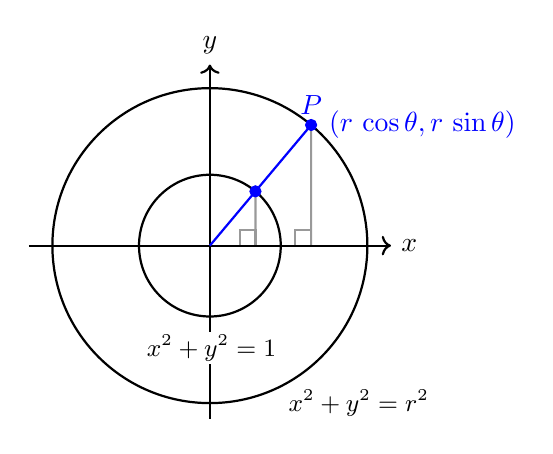
\begin{tikzpicture}
\coordinate(O) at (0,0);
\coordinate(P) at (50:2cm);
\coordinate(Q) at ($ 2*cos(50)*(1,0)$);
\coordinate(R) at (50:0.9cm);
\coordinate(S) at ($ 0.9*cos(50)*(1,0)$);


\draw[gray!80!white, thick] (P) -- (Q);
\draw[gray!80!white, thick] (Q) rectangle ++(-.2,.2);
\draw[gray!80!white, thick] (R) -- (S);
\draw[gray!80!white, thick] (S) rectangle ++(-.2,.2);

\draw[black, thick] (O) circle (2cm);
\draw[black, thick] (O) circle (0.9cm);

\draw[black, thick, ->] (0,-2.2)--(0,2.3) node[above] {$y$};
\draw[black, thick, ->] (-2.3,0)--(2.3,0) node[right] {$x$};

\draw[blue, thick] (O) --(P) node[above , yshift=0] {$P$};
\filldraw[blue] (P) circle (2pt)  node[anchor=west , xshift=3] {($r \, \cos \theta, r \, \sin \theta)$};
\filldraw[blue] (R) circle (2pt);

\node[text width=2cm,fill=white, inner sep=1pt] at (0.2,-1.3)    {\small $x^2+y^2=1$};
\node[text width=2cm] at (2,-2.)    {\small
$x^2+y^2=r^2$};

\end{tikzpicture}
\newline


exam4-2-1
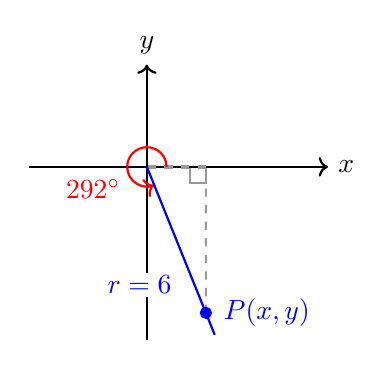
\begin{tikzpicture}
\coordinate(O) at (0,0);
\coordinate(P) at (292:2cm);
\coordinate(Q) at ($ 2*cos(292)*(1,0)$);
\coordinate(R) at (292:2.3cm);

\draw[gray!80!white, thick] (Q) rectangle ++(-.2,-.2);
\draw[gray!80!white, thick, dashed] (P) -- (Q);

\draw[black, thick, ->] (0,-2.2)--(0,1.3) node[above] {$y$};
\draw[black, thick, ->] (-1.5,0)--(2.3,0) node[right] {$x$};
\draw[gray!80!white, ultra thick, dashed] (Q) -- (O);

\draw[red, thick, ->] (0.25,0) arc (0:292:0.25) node[left, midway, yshift=-12] {$\scriptsize 292\degree$};
\draw[blue, thick] (O) --(R) ;
\filldraw[blue] (P) circle (2pt)  node[anchor=west , xshift=3] {$P(x,y)$};

\node[text width=1cm,fill=white, inner sep=1pt] at (0.0,-1.5)    {$\color{blue}\scriptsize r=6$};

\end{tikzpicture}
\newline


exer4-2-1
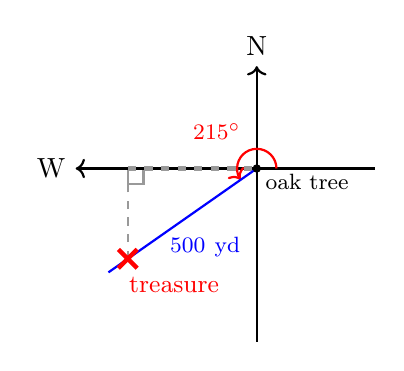
\begin{tikzpicture} [cross/.style={cross out, draw=black, minimum size=2*(#1-\pgflinewidth), inner sep=0pt, outer sep=0pt},cross/.default={5pt}];
\coordinate(O) at (0,0);
\coordinate(P) at (215:2cm);
\coordinate(Q) at ($ 2*cos(215)*(1,0)$);
\coordinate(R) at (215:2.3cm);

\draw[gray!80!white, thick] (Q) rectangle ++(.2,-.2);
\draw[gray!80!white, thick, dashed] (P) -- (Q);

\draw[black, thick, ->] (0,-2.2)--(0,1.3) node[above] {N};
\draw[black, thick, ->] (1.5,0)--(-2.3,0) node[left] {W};
\draw[gray!80!white, ultra thick, dashed] (Q) -- (O);

\draw[red, thick, ->] (0.25,0) arc (0:215:0.25) node[above left, midway, yshift=0] {\footnotesize$ 215\degree$};
\draw[blue, thick] (O) --(R) ;

\node[text width=1.cm,fill=white, inner sep=1pt] at (-.6,-1.)    {\color{blue}\footnotesize 500 yd};
\filldraw[black] (O) circle (1.3pt) node[anchor=north west, xshift=2, yshift=-1, fill=white,inner sep=1pt]{\footnotesize oak tree};
\draw (P) node[cross,red, ultra thick] {};
\node[text width=1.cm, anchor=north west, xshift=-3, yshift=-3] at (P) {\color{red}\small treasure};

\end{tikzpicture}
\newline


fig-4-2-bearings
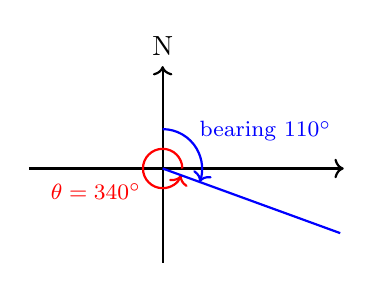
\begin{tikzpicture} 
\coordinate(O) at (0,0);
\coordinate(P) at (340:2.4cm);

\draw[black, thick, ->] (0,-1.2)--(0,1.3) node[above] {N};
\draw[black, thick, ->] (-1.7,0)--(2.3,0);

\draw[red, thick, ->] (0.25,0) arc (0:340:0.25) node[below left, midway, xshift=3, yshift=-3] {\footnotesize$ \theta = 340\degree$};
\draw[blue, thick, ->] (0, 0.5,0) arc (90:-20:0.5) node[above right, midway, xshift=-2, yshift=-2] {\footnotesize bearing $110\degree$};
\draw[blue, thick] (O) --(P) ;

\end{tikzpicture}
\newline


exam-4-2-2
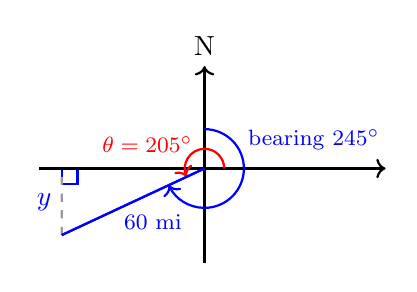
\begin{tikzpicture} 
\coordinate(O) at (0,0);
\coordinate(P) at (205:2.cm);
\coordinate(Q) at ($ 2*cos(205)*(1,0) $);

\draw[blue, thick] (Q) rectangle ++(.2,-.2);
\draw[gray!80!white, thick, dashed] (P)--(Q) node[left, midway] {$\color{blue} y$};
\draw[black, thick, ->] (0,-1.2)--(0,1.3) node[above] {N};
\draw[black, thick, ->] (-2.1,0)--(2.3,0);
\draw[blue, thick] (P)--(O) node[below right, midway, xshift=-7, yshift=-1] {\footnotesize\color{blue} 60 mi};

\draw[red, thick, ->] (0.25,0) arc (0:205:0.25) node[above left, midway, xshift=1, yshift=-5] {\footnotesize$ \theta = 205\degree$};
\draw[blue, thick, ->] (0, 0.5,0) arc (90:-155:0.5) node[right, midway, xshift=0, yshift=18] {\footnotesize bearing $245\degree$};
\draw[blue, thick] (O) --(P) ;

\end{tikzpicture}
\newline


fig-4-2-ferris
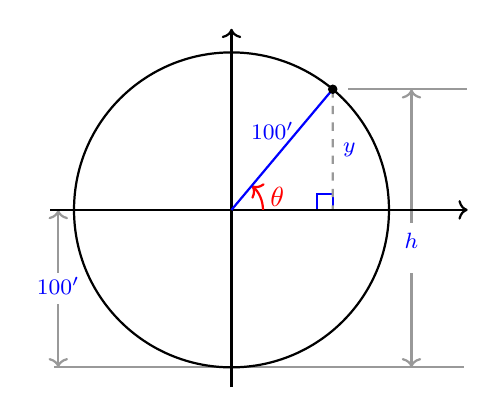
\begin{tikzpicture}
\coordinate(O) at (0,0);
\coordinate(P) at (50:2cm);
\coordinate(Q) at ($ 2*cos(50)*(1,0)$);

\draw[blue, thick] (Q) rectangle ++(-.2,.2);
\draw[gray!80!white, thick, dashed] (P) -- (Q)node[right, midway, color=blue] {\footnotesize $y$};
\draw[gray!80!white, thick, <-] (-2.2,0) -- +(0,-.8) node[below, yshift=2, color=blue] {\footnotesize $100'$};
\draw[gray!80!white, thick, <-] (-2.2,-2) -- +(0,.8) ;
\draw[gray!80!white, thick] (-2.25,-2) -- +(5.2,0);
\draw[gray!80!white, thick] (P)++(.2,0) -- +(1.5,0);
\draw[gray!80!white, thick, <-] (P)++(1,0) -- +(0,-1.7) node[below, color=blue] {\footnotesize $h$};
\draw[gray!80!white, thick, <-] (Q)++(1,-2) -- +(0,1.2) ;

\draw[black, thick, ->] (0,-2.25)--(0,2.3);
\draw[black, thick, ->] (-2.3,0)--(3,0);
\draw[red, thick, ->] (0.4,0) arc (0:50:0.4) node[right, midway] {$\footnotesize \theta$};

\draw[blue, thick] (O) --(P) node[above left, midway, xshift=8, color=blue] {\footnotesize $100'$};

\draw[black, thick] (O) circle (2cm);
\filldraw[black] (P) circle (1.5pt);

\end{tikzpicture}
\newline


fig-4-2-ferris2
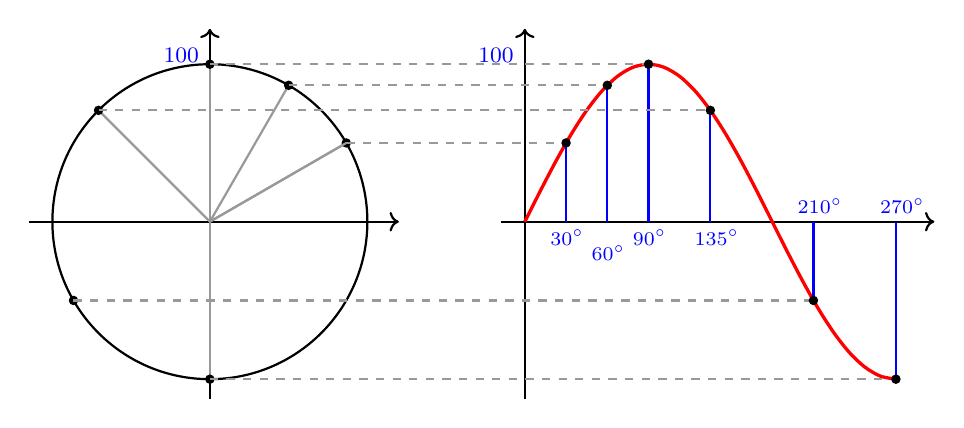
\begin{tikzpicture}
\coordinate(O) at (-4,0);

\draw[black, thick, ->] (O)++(0,-2.25)--++(0,4.7);
\draw[black, thick, ->] (O)++(-2.3,0)--+(4.7,0);

\draw[black, thick, ->] (0,-2.25)--(0,2.45);
\draw[black, thick, ->] (-.3,0)--(5.2,0);
\draw[domain=0:3*pi/2,smooth,variable=\x,red,very thick] plot ({\x},{2*sin(deg(\x))});

\draw[black, thick] (O) circle (2cm);

\coordinate(P) at ($ (O)++2*cos(30)*(1,0)++2*sin(30)*(0,1) $);
\coordinate(Pp) at ($ pi/6*(1,0)++2*sin(30)*(0,1) $);
\coordinate(Po) at ($ pi/6*(1,0) $);
\coordinate(Ph) at ($ (0, -.2)++pi/6*(1,0) $);
\draw[gray!80!white, thick] (P)--(O);
\filldraw[black] (P) circle (1.5pt);
\draw[gray!80!white, thick, dashed] (P)--(Pp);
\draw[blue, thick] (Pp) -- (Po);
\filldraw[black] (Pp) circle (1.5pt);
\node[text width=0.4cm, color=blue] at (Ph) {\scriptsize $30\degree$};

\coordinate(Q) at ($ (O)++2*cos(60)*(1,0)++2*sin(60)*(0,1) $);
\coordinate(Qp) at ($ pi/3*(1,0)++2*sin(60)*(0,1) $);
\coordinate(Qo) at ($ pi/3*(1,0) $);
\coordinate(Qh) at ($ (0, -.4)++pi/3*(1,0) $);
\draw[gray!80!white, thick] (Q)--(O);
\filldraw[black] (Q) circle (1.5pt);
\draw[gray!80!white, thick, dashed] (Q)--(Qp);
\draw[blue, thick] (Qp) -- (Qo);
\filldraw[black] (Qp) circle (1.5pt);
\node[text width=0.4cm, color=blue] at (Qh) {\scriptsize $60\degree$};

\coordinate(R) at ($ (O)++2*(0,1) $);
\coordinate(Rp) at ($ pi/2*(1,0)++2*(0,1) $);
\coordinate(Ro) at ($ pi/2*(1,0) $);
\coordinate(Rh) at ($ (0, -.2)++pi/2*(1,0) $);
\draw[gray!80!white, thick] (R)--(O);
\filldraw[black] (R) circle (1.5pt);
\draw[gray!80!white, thick, dashed] (R)--(Rp);
\draw[blue, thick] (Rp) -- (Ro);
\filldraw[black] (Rp) circle (1.5pt);
\node[text width=0.4cm, color=blue] at (Rh) {\scriptsize $90\degree$};

\coordinate(S) at ($ (O)++2*cos(135)*(1,0)++2*sin(135)*(0,1) $);
\coordinate(Sp) at ($ 3*pi/4*(1,0)++2*sin(135)*(0,1) $);
\coordinate(So) at ($ 3*pi/4*(1,0) $);
\coordinate(Sh) at ($ (0, -.2)++3*pi/4*(1,0) $);
\draw[gray!80!white, thick] (S)--(O);
\filldraw[black] (S) circle (1.5pt);
\draw[gray!80!white, thick, dashed] (S)--(Sp);
\draw[blue, thick] (Sp) -- (So);
\filldraw[black] (Sp) circle (1.5pt);
\node[text width=0.4cm, color=blue] at (Sh) {\scriptsize $135\degree$};

\coordinate(T) at ($ (O)++2*cos(210)*(1,0)++2*sin(210)*(0,1) $);
\coordinate(Tp) at ($ 7*pi/6*(1,0)++2*sin(210)*(0,1) $);
\coordinate(To) at ($ 7*pi/6*(1,0) $);
\coordinate(Th) at ($ (0, .2)++7*pi/6*(1,0) $);
\draw[gray!80!white, thick] (P)--(O);
\filldraw[black] (T) circle (1.5pt);
\draw[gray!80!white, thick, dashed] (T)--(Tp);
\draw[blue, thick] (Tp) -- (To);
\filldraw[black] (Tp) circle (1.5pt);
\node[text width=0.4cm, color=blue] at (Th) {\scriptsize $210\degree$};

\coordinate(U) at ($ (O)++2*(0,-1) $);
\coordinate(Up) at ($ 3*pi/2*(1,0)++2*(0,-1) $);
\coordinate(Uo) at ($ 3*pi/2*(1,0) $);
\coordinate(Uh) at ($ (0, .2)++3*pi/2*(1,0) $);
\draw[gray!80!white, thick] (U)--(O);
\filldraw[black] (U) circle (1.5pt);
\draw[gray!80!white, thick, dashed] (U)--(Up);
\draw[blue, thick] (Up) -- (Uo);
\filldraw[black] (Up) circle (1.5pt);
\node[text width=0.4cm, color=blue] at (Uh) {\scriptsize $270\degree$};

\node[text width=0.5cm, anchor=south east, xshift=1, yshift=-3, color=blue] at (R) {\footnotesize 100};

\node[text width=0.5cm, anchor=south east, xshift=1, yshift=-3, color=blue] at (0,2) {\footnotesize 100};

\end{tikzpicture}
\newline


fig-4-2-ferris3
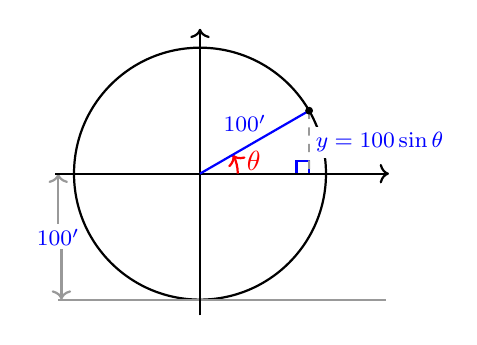
\begin{tikzpicture} [scale=.8]
\coordinate(O) at (0,0);
\coordinate(P) at (30:2cm);
\coordinate(Q) at ($ 2*cos(30)*(1,0)$);

\draw[black, thick] (O) circle (2cm);
\draw[blue, thick] (Q) rectangle ++(-.2,.2);
\draw[gray!80!white, thick, dashed] (P) -- (Q)node[right, midway, color=blue,fill=white, inner sep=2pt] {\footnotesize $y=100 \sin \theta$};
\draw[gray!80!white, thick, <-] (-2.25,0) -- +(0,-.8) node[below, yshift=2, color=blue] {\footnotesize $100'$};
\draw[gray!80!white, thick, <-] (-2.2,-2) -- +(0,.8) ;
\draw[gray!80!white, thick] (-2.25,-2) -- +(5.2,0);

\draw[black, thick, ->] (0,-2.25)--(0,2.3);
\draw[black, thick, ->] (-2.3,0)--(3,0);
\draw[red, thick, ->] (0.6,0) arc (0:30:0.6) node[right, midway, yshift=1] {$\footnotesize \theta$};

\draw[blue, thick] (O) --(P) node[above left, midway, xshift=8, color=blue] {\footnotesize $100'$};

\filldraw[black] (P) circle (1.5pt);

\end{tikzpicture}
\newline


exam4-2-3a
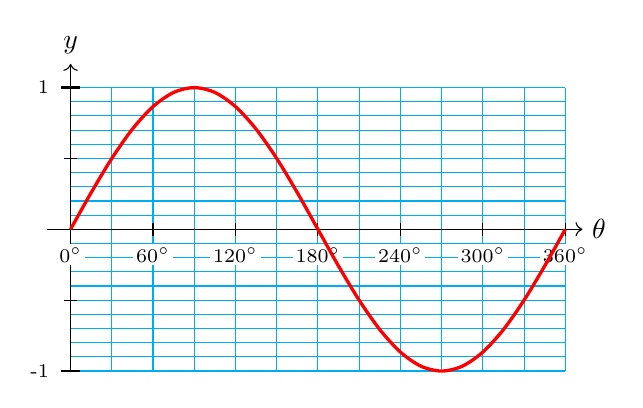
\begin{tikzpicture}

\draw[cyan,xstep=pi/6,ystep=0.18]
(0,-1.8) grid (2*pi,1.8);

\draw[->] (-.3,0) -- (6.5,0) node[right] {$\theta$};
\draw[->] (0,-1.8) -- (0,2.1) node[above] {$y$};

\foreach \x [evaluate=\x as \xi using int( 60* \x )] in {0,1,...,6}
\draw[black] ($ pi*\x /3*(1,0) +(0,.08) $) --++(0,-.16) node[anchor=north, xshift=0,yshift=-3, fill=white, inner sep=1pt] {\scriptsize$ \xi \degree$};
\foreach \y in {-0.9, 0.9}
\draw[black] (.08,\y ) --++(-.16,0);
\foreach \y in {-1,1}
\draw[black, thick] (.12,1.8*\y ) --++(-.24,0) node[anchor=east, xshift=-3, fill=white, inner sep=1pt] {\scriptsize\y};

\draw[domain=0:2*pi,smooth,variable=\x,red,very thick] plot ({\x},{1.8*sin(deg(\x))});

\end{tikzpicture}
\newline


exam4-2-3b

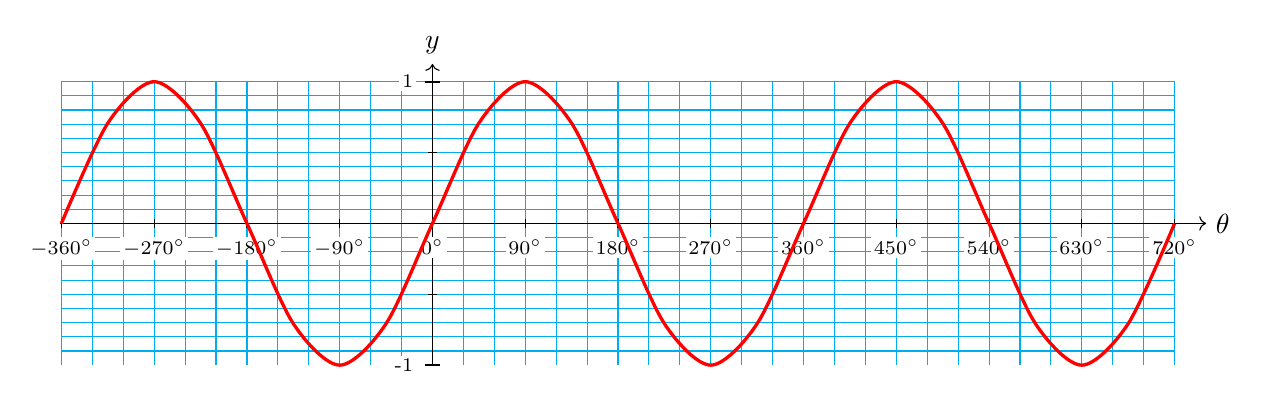
\begin{tikzpicture} [scale=.75]

\draw[cyan,xstep=pi/6,ystep=0.24]
(-2*pi,-2.4) grid (4*pi,2.4);

\draw[->] (-6.3,0) -- (13.1,0) node[right] {$\theta$};
\draw[->] (0,-2.4) -- (0,2.7) node[above] {$y$};

\foreach \x [evaluate=\x as \xi using int( 90* \x )] in {-4,-3,...,8}
\draw[black] ($ pi*\x /2*(1,0) +(0,.08) $) --++(0,-.16) node[anchor=north, xshift=0,yshift=-3, fill=white, inner sep=1pt] {\scriptsize$ \xi \degree$};
\foreach \y in {-1.2, 1.2}
\draw[black] (.08,\y ) --++(-.16,0);
\foreach \y in {-1,1}
\draw[black, thick] (.12,2.4*\y ) --++(-.24,0) node[anchor=east, xshift=-3, fill=white, inner sep=1pt] {\scriptsize\y};

\draw[domain=-2*pi:4*pi,smooth,variable=\x,red,very thick] plot ({\x},{2.4*sin(deg(\x))});

\end{tikzpicture}
\newline



exer4-2-3 grid

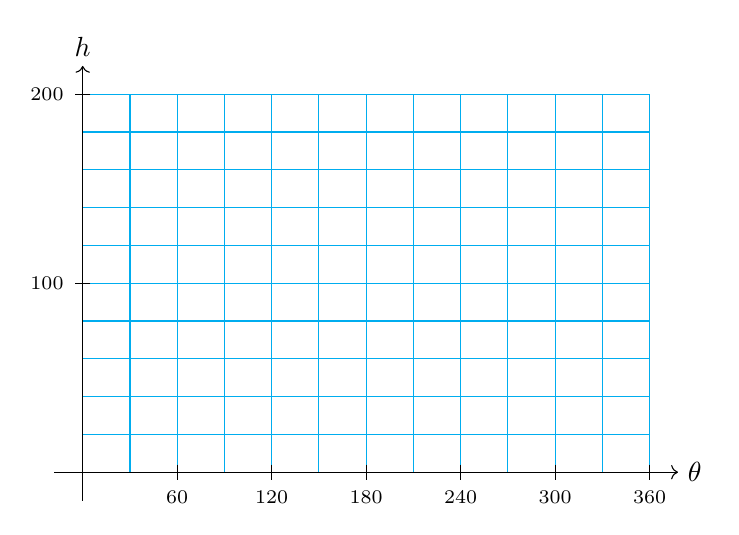
\begin{tikzpicture} [scale=1.2]
\draw[cyan,xstep=0.5,ystep=0.4]
(0,0) grid (6,4);

\draw[->] (-.3,0) -- (6.3,0) node[right] {$\theta$};
\draw[->] (0,-.3) -- (0,4.3) node[above] {$h$};

\foreach \x [evaluate=\x as \xi using int( 60* \x )] in {1,2,...,6}
\draw[black] ($ \x *(1,0) +(0,.08) $) --++(0,-.16) node[anchor=north, xshift=0,yshift=-3, fill=white, inner sep=1pt] {\scriptsize$ \xi $};

\foreach \y  [evaluate=\y as \yi using int( 50* \y )] in {2,4}
\draw[black] (.08,\y ) --++(-.16,0) node[anchor=east, xshift=-3, fill=white, inner sep=1pt] {\scriptsize\yi};

\end{tikzpicture}
\newline


exer4-2-3ans

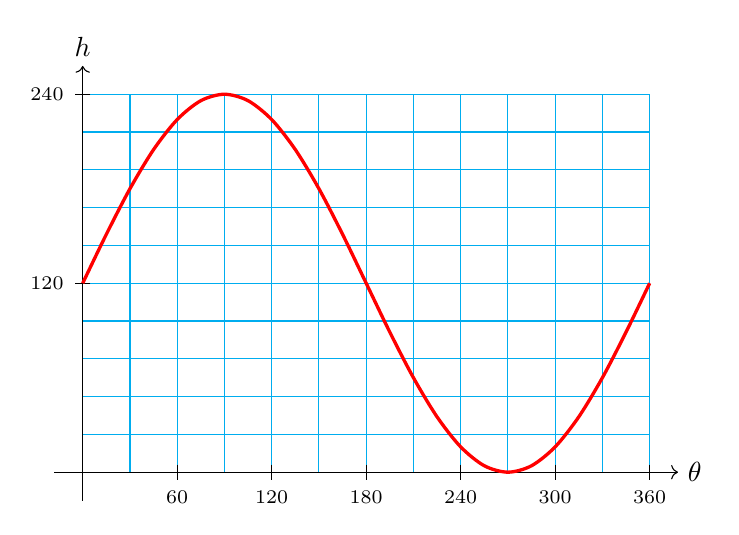
\begin{tikzpicture} [scale=1.2]
\draw[cyan,xstep=0.5,ystep=0.4]
(0,0) grid (6,4);

\draw[->] (-.3,0) -- (6.3,0) node[right] {$\theta$};
\draw[->] (0,-.3) -- (0,4.3) node[above] {$h$};

\foreach \x [evaluate=\x as \xi using int( 60* \x )] in {1,2,...,6}
\draw[black] ($ \x *(1,0) +(0,.08) $) --++(0,-.16) node[anchor=north, xshift=0,yshift=-3, fill=white, inner sep=1pt] {\scriptsize$ \xi $};

\foreach \y  [evaluate=\y as \yi using int( 60* \y )] in {2,4}
\draw[black] (.08,\y ) --++(-.16,0) node[anchor=east, xshift=-3, fill=white, inner sep=1pt] {\scriptsize\yi};

\draw[domain=0:6,smooth,variable=\x,red,very thick] plot ({\x},{2+2*sin(pi/3*deg(\x))});

\end{tikzpicture}
\newline

IGNORE THIS ONE
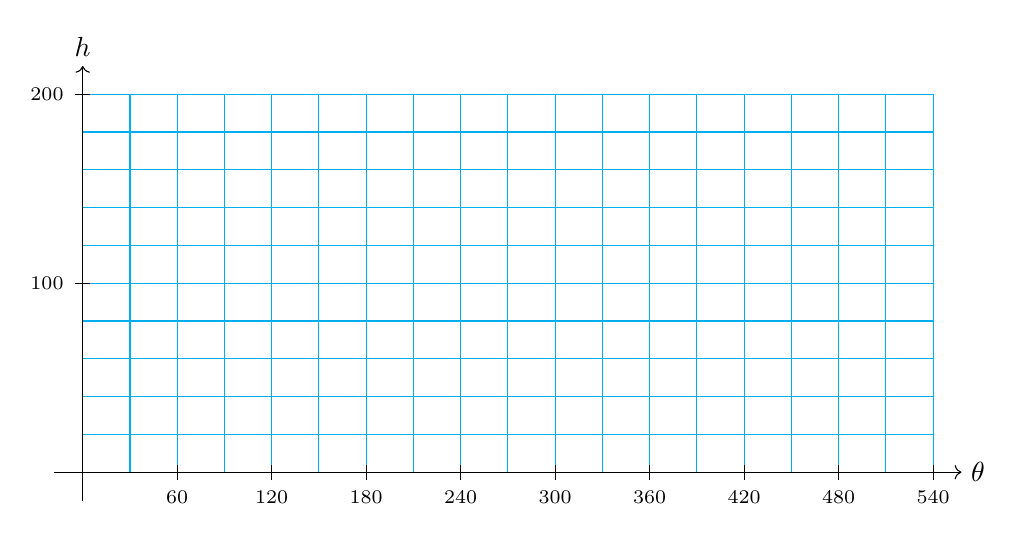
\begin{tikzpicture} [scale=1.2]
\draw[cyan,xstep=0.5,ystep=0.4]
(0,0) grid (9,4);

\draw[->] (-.3,0) -- (9.3,0) node[right] {$\theta$};
\draw[->] (0,-.3) -- (0,4.3) node[above] {$h$};

\foreach \x [evaluate=\x as \xi using int( 60* \x )] in {1,2,...,9}
\draw[black] ($ \x *(1,0) +(0,.08) $) --++(0,-.16) node[anchor=north, xshift=0,yshift=-3, fill=white, inner sep=1pt] {\scriptsize$ \xi $};

\foreach \y  [evaluate=\y as \yi using int( 50* \y )] in {2,4}
\draw[black] (.08,\y ) --++(-.16,0) node[anchor=east, xshift=-3, fill=white, inner sep=1pt] {\scriptsize\yi};

\end{tikzpicture}
\newline

exam4-2-4a circle
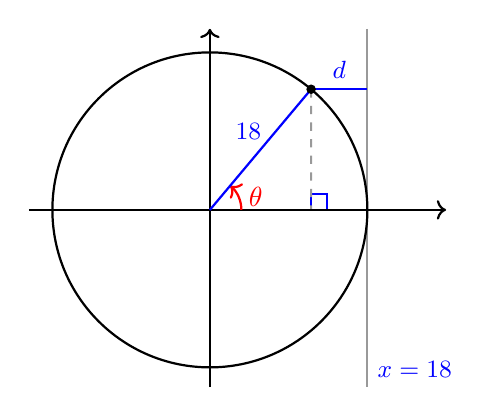
\begin{tikzpicture}
\coordinate(O) at (0,0);
\coordinate(P) at (50:2cm);
\coordinate(Q) at ($ 2*cos(50)*(1,0)$);
\coordinate(R) at ($ (2,0) ++2*sin(50)*(0,1)$);

\draw[blue, thick] (Q) rectangle ++(.2,.2);
\draw[gray!80!white, thick, dashed] (P) -- (Q);

\draw[gray!80!white, thick] (2,2.3) -- (2, -2.25) node[below right, yshift=13, color=blue] {\small $x=18$};
\draw[blue, thick] (P) -- (R) node[above, midway] {\small $d$};

\draw[black, thick, ->] (0,-2.25)--(0,2.3);
\draw[black, thick, ->] (-2.3,0)--(3,0);
\draw[red, thick, ->] (0.4,0) arc (0:50:0.4) node[right, midway] {$\footnotesize \theta$};

\draw[blue, thick] (O) --(P) node[above left, midway, xshift=4, color=blue] {\small $18$};

\draw[black, thick] (O) circle (2cm);
\filldraw[black] (P) circle (1.5pt);

\end{tikzpicture}
\newline


exam4-2-4b transformed cosine graph

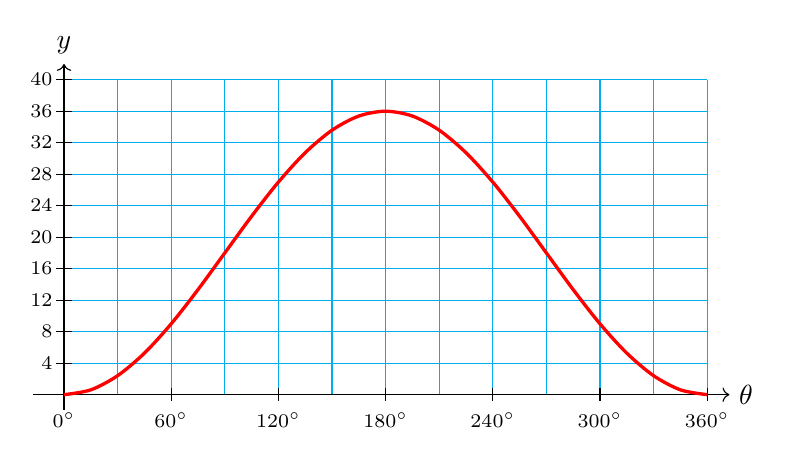
\begin{tikzpicture} [xscale=1.3]

\draw[cyan,xstep=pi/6,ystep=0.4] (0,0) grid (2*pi,4);

\draw[->] (-.3,0) -- (6.5,0) node[right] {$\theta$};
\draw[->] (0,-0.3) -- (0,4.2) node[above] {$y$};

\foreach \x [evaluate=\x as \xi using int( 60* \x )] in {0,1,...,6}
\draw[black] ($ pi*\x /3*(1,0) +(0,.08) $) --++(0,-.16) node[anchor=north, xshift=0,yshift=-3, fill=white, inner sep=1pt] {\scriptsize$ \xi \degree$};
\foreach \y [evaluate=\y as \yi using int(10* \y )] in {.401, .801,..., 4.01}
\draw[black] (.08,\y ) --++(-.16,0) node[anchor=east, xshift=0,yshift=0, fill=white, inner sep=1pt] {\scriptsize$ \yi $};

\draw[domain=0:2*pi,smooth,variable=\x,red,very thick] plot ({\x},{1.8-1.8*cos(deg(\x))});

\end{tikzpicture}
\newline



exer4-2-4 grid

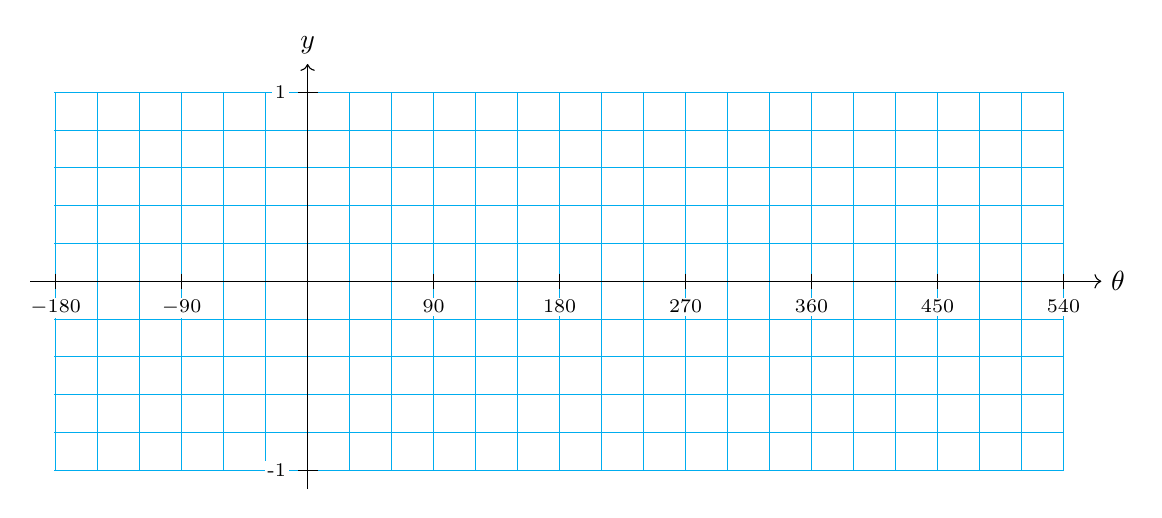
\begin{tikzpicture} [xscale=1.6, yscale=1.2]
\draw[cyan,xstep=0.3333, ystep=0.4]
(-2.01,-2) grid (6,2);

\draw[->] (-2.2,0) -- (6.3,0) node[right] {$\theta$};
\draw[->] (0,-2.2) -- (0,2.3) node[above] {$y$};

\foreach \x [evaluate=\x as \xi using int( 90* \x )] in {1,2,...,6}
\draw[black] ($ \x *(1,0) +(0,.08) $) --++(0,-.16) node[anchor=north, xshift=0,yshift=-3, fill=white, inner sep=1pt] {\scriptsize$ \xi $};
\foreach \x [evaluate=\x as \xi using int( 90* \x )] in {-2,-1}
\draw[black] ($ \x *(1,0) +(0,.08) $) --++(0,-.16) node[anchor=north, xshift=0,yshift=-3, fill=white, inner sep=1pt] {\scriptsize$ \xi $};

\foreach \y  [evaluate=\y as \yi using int(  \y /2 )] in {-2,2}
\draw[black] (.08,\y ) --++(-.16,0) node[anchor=east, xshift=-3, fill=white, inner sep=1pt] {\scriptsize\yi};

\end{tikzpicture}
\newline


exer4-2-4ans graph

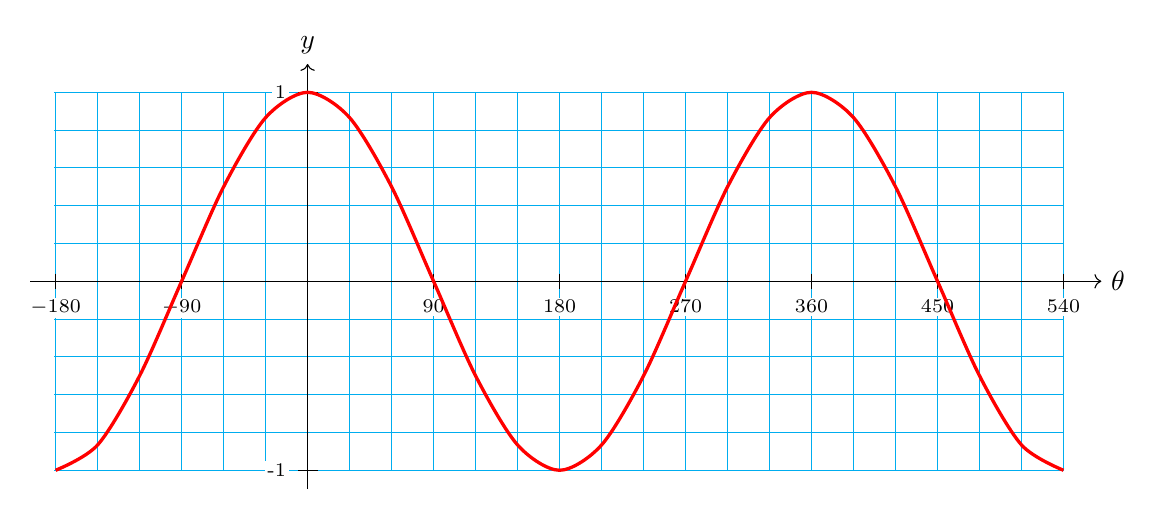
\begin{tikzpicture} [xscale=1.6, yscale=1.2]
\draw[cyan,xstep=0.3333, ystep=0.4]
(-2.01,-2) grid (6,2);

\draw[->] (-2.2,0) -- (6.3,0) node[right] {$\theta$};
\draw[->] (0,-2.2) -- (0,2.3) node[above] {$y$};

\foreach \x [evaluate=\x as \xi using int( 90* \x )] in {1,2,...,6}
\draw[black] ($ \x *(1,0) +(0,.08) $) --++(0,-.16) node[anchor=north, xshift=0,yshift=-3, fill=white, inner sep=1pt] {\scriptsize$ \xi $};
\foreach \x [evaluate=\x as \xi using int( 90* \x )] in {-2,-1}
\draw[black] ($ \x *(1,0) +(0,.08) $) --++(0,-.16) node[anchor=north, xshift=0,yshift=-3, fill=white, inner sep=1pt] {\scriptsize$ \xi $};

\foreach \y  [evaluate=\y as \yi using int(  \y /2 )] in {-2,2}
\draw[black] (.08,\y ) --++(-.16,0) node[anchor=east, xshift=-3, fill=white, inner sep=1pt] {\scriptsize\yi};

\draw[domain=-2:6,smooth,variable=\x,red,very thick] plot ({\x},{2* cos(deg(\x*pi/2))});
\end{tikzpicture}
\newline



exam4-2-5 semi-circle graph

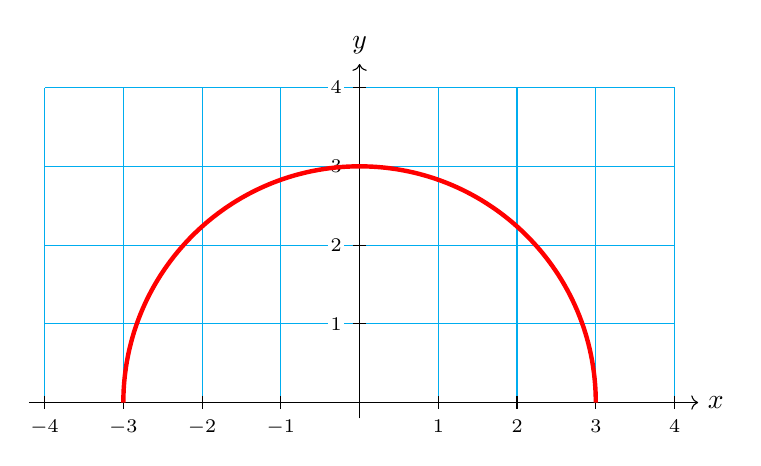
\begin{tikzpicture} 
\draw[cyan] (-4,0) grid (4,4);

\draw[->] (-4.2,0) -- (4.3,0) node[right] {$x$};
\draw[->] (0,-.2) -- (0,4.3) node[above] {$y$};

\foreach \x  in {-4, -3, ..., -1, 1,2,...,4}
\draw[black] ($ \x *(1,0) +(0,.08) $) --++(0,-.16) node[anchor=north, xshift=0,yshift=-3, fill=white, inner sep=1pt] {\scriptsize$ \x $};

\foreach \y  in {1,2, 3, 4}
\draw[black] (.08,\y ) --++(-.16,0) node[anchor=east, xshift=-3, fill=white, inner sep=1pt] {\scriptsize\y};

\draw[red, ultra thick] (3,0) arc (0:180:3);

\end{tikzpicture}
\newline



fig-4-2-caut1 angle

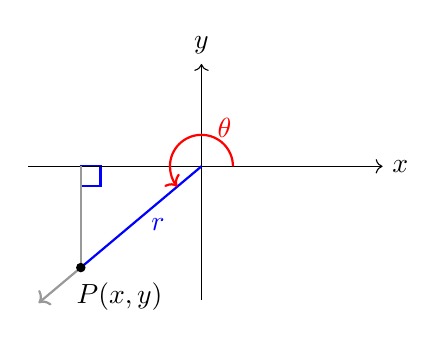
\begin{tikzpicture} 
\coordinate(O) at (0,0);
\coordinate(P) at (220:2cm);
\coordinate(Pp) at (220:2.7cm);
\coordinate(Q) at ($ 2*cos(220)*(1,0)$);

\draw[blue, thick] (Q) rectangle +(.25, -.25);

\draw[->] (-2.2,0) -- (2.3,0) node[right] {$x$};
\draw[->] (0,-1.7) -- (0,1.3) node[above] {$y$};

\draw[blue, thick] (O) -- (P) node[below right, midway, yshift = 3] {$r$};
\draw[gray!80!white, thick, ->] (P) -- (Pp);
\draw[gray!80!white, thick] (Q)--(P);
\filldraw[black] (P) circle (1.5pt) node[anchor=north, xshift=14, yshift=-2] {$P(x,y)$};

\draw[red, thick, ->] (.4,0) arc (0:220:.4) node[above right, midway, xshift=6, yshift=-4]{$\theta$};

\end{tikzpicture}
\newline



fig-4-2-caut2b angle on unit circle

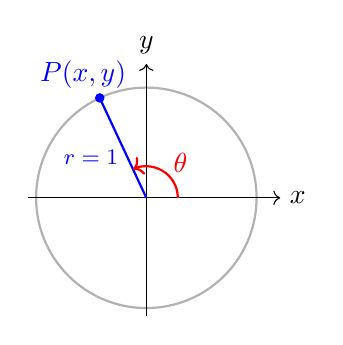
\begin{tikzpicture} 
\coordinate(O) at (0,0);
\coordinate(P) at (115:1.4cm);

\draw[gray!60!white, thick] (O) circle (1.4cm);

\draw[->] (-1.5,0) -- (1.7,0) node[right] {$x$};
\draw[->] (0,-1.5) -- (0,1.7) node[above] {$y$};

\draw[blue, thick] (O) -- (P) node[below left, midway, xshift=2, yshift = 3] {\footnotesize $r=1$};
\filldraw[blue] (P) circle (1.5pt) node[anchor=south, xshift=-6] {$P(x,y)$};

\draw[red, thick, ->] (.4,0) arc (0:115:.4) node[above right, midway, xshift=0, yshift=-4]{$\theta$};

\end{tikzpicture}
\newline


fig-4-2-caut2cos cosine graph

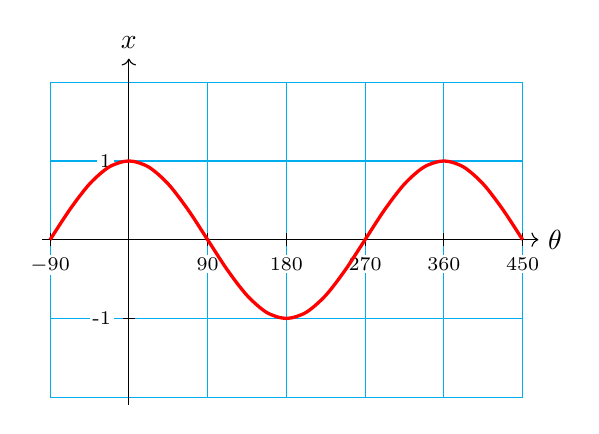
\begin{tikzpicture} 
\draw[cyan] (-1,-2) grid (5,2);

\draw[->] (-1.1,0) -- (5.2,0) node[right] {$\theta$};
\draw[->] (0,-2.1) -- (0,2.3) node[above] {$x$};
\foreach \x [evaluate=\x as \xi using int( 90* \x )] in {-1,1,2,...,5}
\draw[black] ($ \x *(1,0) +(0,.08) $) --++(0,-.16) node[anchor=north, xshift=0,yshift=-3, fill=white, inner sep=1pt] {\scriptsize$ \xi $};

\foreach \y   in {-1,1} \draw[black] (.08,\y ) --++(-.16,0) node[anchor=east, xshift=-3, fill=white, inner sep=1pt] {\scriptsize\y};

\draw[domain=-1:5,smooth,variable=\x,red,very thick] plot ({\x},{cos(pi/2*deg(\x))});

\end{tikzpicture}
\newline


fig-4-2-caut2sin sine graph

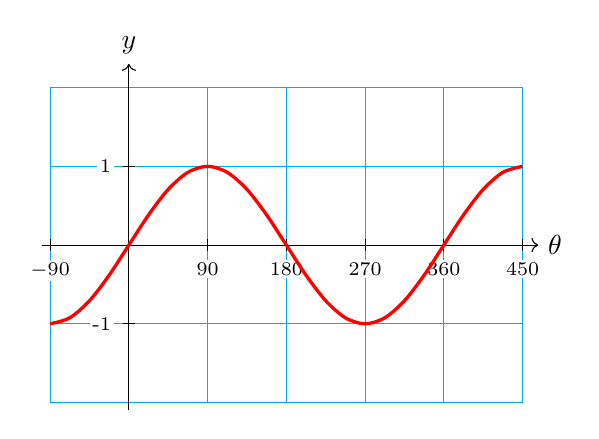
\begin{tikzpicture} 
\draw[cyan] (-1,-2) grid (5,2);

\draw[->] (-1.1,0) -- (5.2,0) node[right] {$\theta$};
\draw[->] (0,-2.1) -- (0,2.3) node[above] {$y$};
\foreach \x [evaluate=\x as \xi using int( 90* \x )] in {-1,1,2,...,5}
\draw[black] ($ \x *(1,0) +(0,.08) $) --++(0,-.16) node[anchor=north, xshift=0,yshift=-3, fill=white, inner sep=1pt] {\scriptsize$ \xi $};

\foreach \y   in {-1,1} \draw[black] (.08,\y ) --++(-.16,0) node[anchor=east, xshift=-3, fill=white, inner sep=1pt] {\scriptsize\y};

\draw[domain=-1:5,smooth,variable=\x,red,very thick] plot ({\x},{sin(pi/2*deg(\x))});

\end{tikzpicture}
\newline


exer4-2-5ansa sine graph

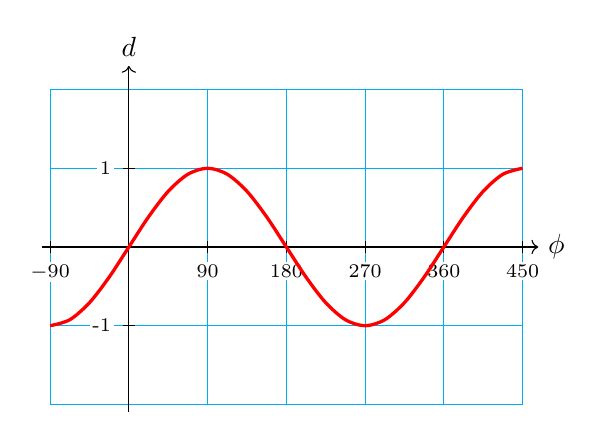
\begin{tikzpicture} 
\draw[cyan] (-1,-2) grid (5,2);

\draw[->] (-1.1,0) -- (5.2,0) node[right] {$\phi$};
\draw[->] (0,-2.1) -- (0,2.3) node[above] {$d$};
\foreach \x [evaluate=\x as \xi using int( 90* \x )] in {-1,1,2,...,5}
\draw[black] ($ \x *(1,0) +(0,.08) $) --++(0,-.16) node[anchor=north, xshift=0,yshift=-3, fill=white, inner sep=1pt] {\scriptsize$ \xi $};

\foreach \y   in {-1,1} \draw[black] (.08,\y ) --++(-.16,0) node[anchor=east, xshift=-3, fill=white, inner sep=1pt] {\scriptsize\y};

\draw[domain=-1:5,smooth,variable=\x,red,very thick] plot ({\x},{sin(pi/2*deg(\x))});

\end{tikzpicture}
\newline


exer4-2-5ansb cosine graph

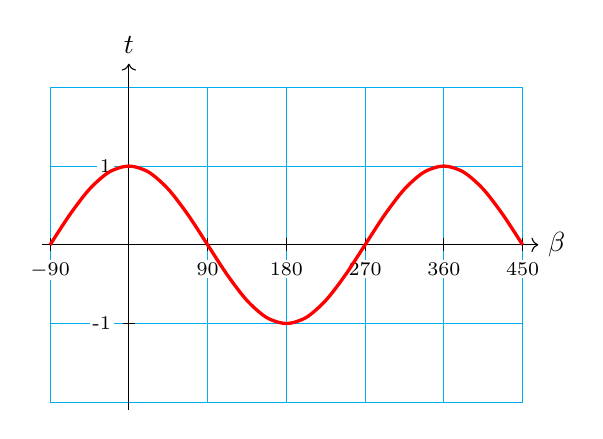
\begin{tikzpicture} 
\draw[cyan] (-1,-2) grid (5,2);

\draw[->] (-1.1,0) -- (5.2,0) node[right] {$\beta$};
\draw[->] (0,-2.1) -- (0,2.3) node[above] {$t$};
\foreach \x [evaluate=\x as \xi using int( 90* \x )] in {-1,1,2,...,5}
\draw[black] ($ \x *(1,0) +(0,.08) $) --++(0,-.16) node[anchor=north, xshift=0,yshift=-3, fill=white, inner sep=1pt] {\scriptsize$ \xi $};

\foreach \y   in {-1,1} \draw[black] (.08,\y ) --++(-.16,0) node[anchor=east, xshift=-3, fill=white, inner sep=1pt] {\scriptsize\y};

\draw[domain=-1:5,smooth,variable=\x,red,very thick] plot ({\x},{cos(pi/2*deg(\x))});

\end{tikzpicture}
\newline


SKIP THIS: fig-4-2-tan slopes
It is the figure used in hmwk 2.2.53 hp2-2-53.svg

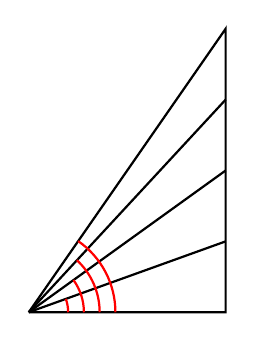
\begin{tikzpicture} 
\coordinate(O) at (0,0);
\coordinate(A) at (2.5,0);
\coordinate(B) at (2.5,0.9);
\coordinate(C) at (2.5,1.8);
\coordinate(D) at (2.5,2.7);
\coordinate(E) at (2.5,3.6);

[draw[blue, thick] (A) rectangle (-.25,.25);

\draw[black, thick] (O) -- (A) --(E)--(O);
\draw[black, thick] (O) -- (B);
\draw[black, thick] (O) -- (C);
\draw[black, thick] (O) -- (D);

\draw[red, thick] (0.5, 0) arc(0:{atan(9/25)}:0.5);
\draw[red, thick] (0.7, 0) arc(0:{atan(18/25)}:0.7);
\draw[red, thick] (0.9, 0) arc(0:{atan(27/25)}:0.9);
\draw[red, thick] (1.1, 0) arc(0:{atan(36/25)}:1.1);

\end{tikzpicture}
\newline


exam4-2-6a tangent graph

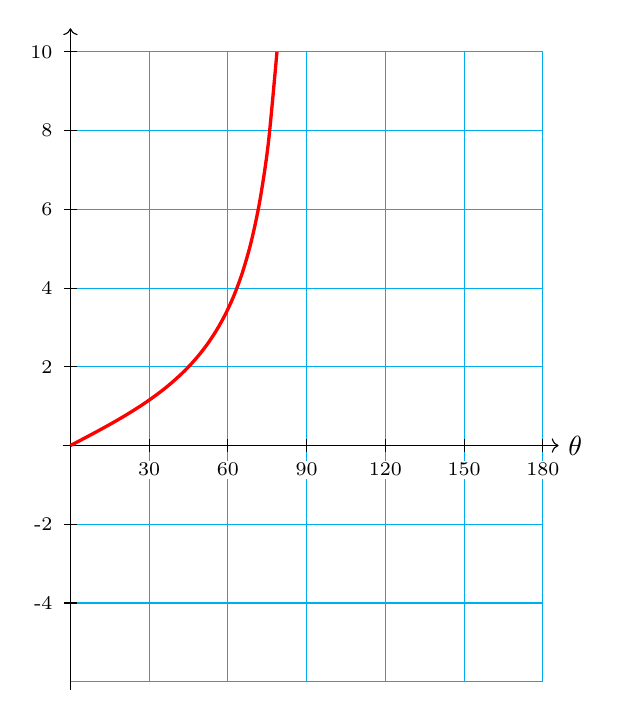
\begin{tikzpicture} 
\draw[cyan] (0,-3) grid (6,5);

\draw[->] (-.1,0) -- (6.2,0) node[right] {$\theta$};
\draw[->] (0,-3.1) -- (0,5.3);
\foreach \x [evaluate=\x as \xi using int( 30* \x )] in {1,2,...,6}
\draw[black] ($ \x *(1,0) +(0,.08) $) --++(0,-.16) node[anchor=north, xshift=0,yshift=-3, fill=white, inner sep=1pt] {\scriptsize$ \xi $};

\foreach \y [evaluate=\y as \yi using int( 2* \y )]   in {-2,-1,1,2,...,5} \draw[black] (.08,\y ) --++(-.16,0) node[anchor=east, xshift=-3, fill=white, inner sep=1pt] {\scriptsize\yi};

\draw[domain={0:atan(5)/30},smooth,variable=\x,red,very thick] plot ({\x},{tan(30*\x)});

\end{tikzpicture}
\newline



exam4-2-6b supplementary angles

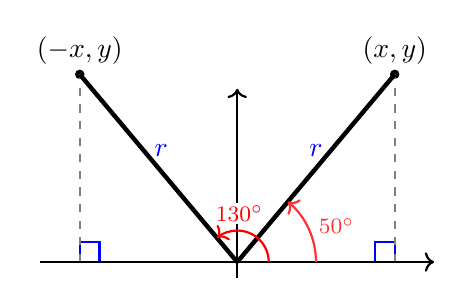
\begin{tikzpicture} 
\coordinate(A) at (2,0);
\coordinate (B) at ($ (2,0)++2*tan(50)*(0,1)  $);
\coordinate(Ap) at (-2,0);
\coordinate (Bp) at ($ (-2,0)++2*tan(50)*(0,1)  $);
\coordinate (O) at (0,0);

\filldraw[black] (B) circle (1.5pt) node[anchor=south] {$(x,y)$};
\draw[blue,thick] (A) rectangle +(-0.25,0.25);
\draw[gray,thick, dashed] (A)--(B);
\draw[black, ultra thick] (O)--(B) node[above,midway] {\color{blue}$r$};

\filldraw[black] (Bp) circle (1.5pt) node[anchor=south] {$(-x,y)$};
\draw[blue,thick] (Ap) rectangle +(0.25,0.25);
\draw[gray,thick, dashed] (Ap)--(Bp);
\draw[black, ultra thick] (O)--(Bp) node[above,midway, xshift=1] {\color{blue}$r$};

\draw[black,thick,->] (-2.5,0) -- (2.5,0);
\draw[black,thick,->] (0,-.2) -- (0,2.2) ;

\draw[red!80!white,thick,->] (1,0) arc (0:50:1) node[right, midway, xshift=0, yshift=1] {\footnotesize$50\degree$};
\draw[red,thick,->] (.4,0) arc (0:130:.4) node[above, midway, xshift=-4, yshift=3,fill=white, inner sep=1pt] {\footnotesize$130\degree$};
\end{tikzpicture}
\newline


exam4-2-6c tangent graph

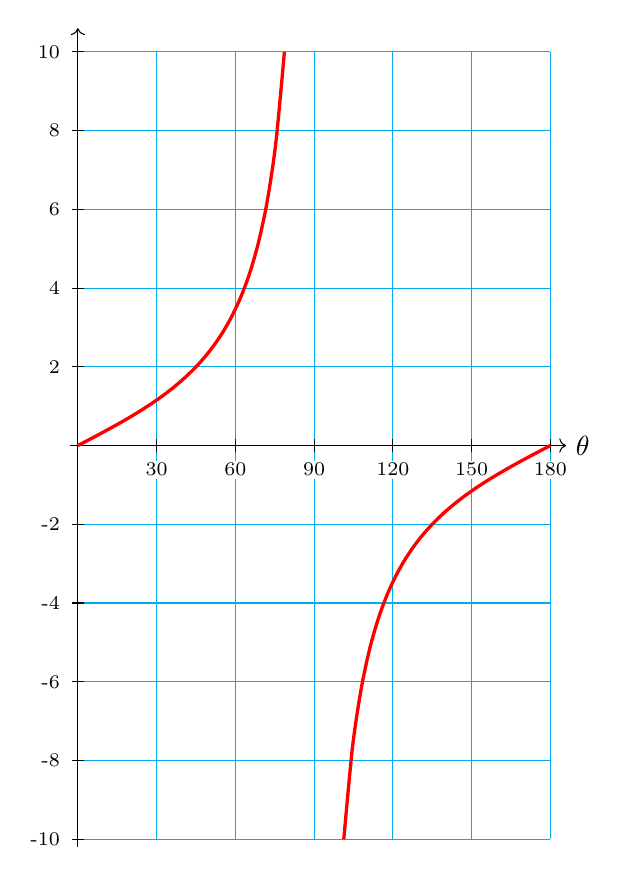
\begin{tikzpicture} 
\draw[cyan] (0,-5) grid (6,5);

\draw[->] (-.1,0) -- (6.2,0) node[right] {$\theta$};
\draw[->] (0,-5.1) -- (0,5.3);
\foreach \x [evaluate=\x as \xi using int( 30* \x )] in {1,2,...,6}
\draw[black] ($ \x *(1,0) +(0,.08) $) --++(0,-.16) node[anchor=north, xshift=0,yshift=-3, fill=white, inner sep=1pt] {\scriptsize$ \xi $};

\foreach \y [evaluate=\y as \yi using int( 2* \y )]   in {-5,-4,...,-1,1,2,...,5} \draw[black] (.08,\y ) --++(-.16,0) node[anchor=east, xshift=-3, fill=white, inner sep=1pt] {\scriptsize\yi};

\draw[domain={0:atan(5)/30},smooth,variable=\x,red,very thick] plot ({\x},{tan(30*\x)});

\draw[domain={atan(-5)/30+6:6},smooth,variable=\x,red,very thick] plot ({\x},{tan(30*\x)});

\end{tikzpicture}
\newline


exam4-2-6d angles differing by 180 degrees

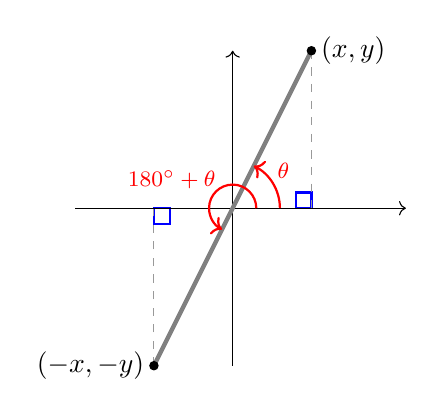
\begin{tikzpicture} 
\coordinate (O) at (0,0);
\coordinate (B) at (1,0);
\coordinate (A) at (1,2);
\coordinate (Bp) at (-1,0);
\coordinate (Ap) at (-1,-2);

\draw[blue, thick] (B) rectangle +(-.2,.2);
\draw[blue, thick] (Bp) rectangle +(.2,-.2);

\draw[gray!80!white, dashed] (A)--(B);
\draw[gray!80!white, dashed] (Ap)--(Bp);

\draw[->] (-2,0) -- (2.2,0);
\draw[->] (0,-2) -- (0,2);

\draw[gray, ultra thick] (A) -- (Ap);
\filldraw[black] (A) circle (1.5pt) node[anchor=west] {$(x,y)$};
\filldraw[black] (Ap) circle (1.5pt) node[anchor=east] {$(-x,-y)$};

\draw[red, thick, ->] (0.3,0) arc(0:{atan(2)+180}:.3) node[below  left, midway, xshift=2, yshift=10] {\footnotesize $180\degree + \theta$};
\draw[red, thick, ->] (0.6,0) arc(0:{atan(2)}:.6) node[above  right, midway, xshift=-2, yshift=-2] {\footnotesize $\theta$};
\end{tikzpicture}
\newline


exam4-2-6d2 angles differing by 180 degrees

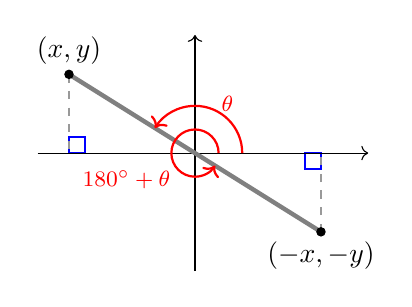
\begin{tikzpicture} 
\coordinate (O) at (0,0);
\coordinate (B) at (1.6,0);
\coordinate (A) at (1.6,-1);
\coordinate (Bp) at (-1.6,0);
\coordinate (Ap) at (-1.6,1);

\draw[blue, thick] (B) rectangle +(-.2,-.2);
\draw[blue, thick] (Bp) rectangle +(.2,.2);

\draw[gray!80!white, dashed] (A)--(B);
\draw[gray!80!white, dashed] (Ap)--(Bp);

\draw[->] (-2,0) -- (2.2,0);
\draw[->] (0,-1.5) -- (0,1.5);

\draw[gray, ultra thick] (A) -- (Ap);
\filldraw[black] (A) circle (1.5pt) node[anchor=north] {$(-x,-y)$};
\filldraw[black] (Ap) circle (1.5pt) node[anchor=south] {$(x,y)$};

\draw[red, thick, ->] (0.3,0) arc(0:{360-atan(1/1.6)}:.3) node[below left, midway, xshift=3, yshift=-5] {\footnotesize $180\degree + \theta$};
\draw[red, thick, ->] (0.6,0) arc(0:{180-atan(1/1.6)}:.6) node[above, midway, xshift=7, yshift=-5] {\footnotesize $\theta$};
\end{tikzpicture}
\newline


exam4-2-6e tangent graph

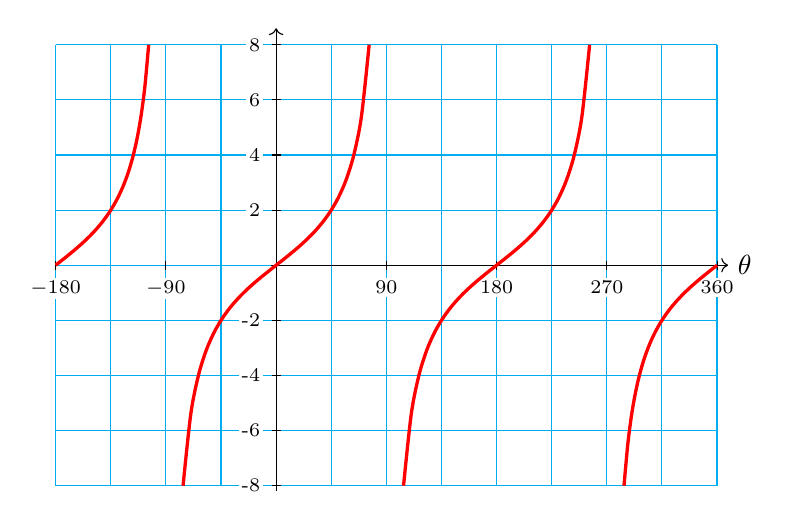
\begin{tikzpicture} [scale=.7]
\draw[cyan] (-4,-4) grid (8,4);

\draw[->] (-.1,0) -- (8.2,0) node[right] {$\theta$};
\draw[->] (0,-4.1) -- (0,4.3);
\foreach \x [evaluate=\x as \xi using int( 45* \x )] in {-4, -2, 2, 4,6,8} \draw[black] ($ \x *(1,0) +(0,.08) $) --++(0,-.16) node[anchor=north, xshift=0,yshift=-3, fill=white, inner sep=1pt] {\scriptsize$ \xi $};

\foreach \y [evaluate=\y as \yi using int( 2* \y )]   in {-4,-3,...,-1,1,2,...,4} \draw[black] (.08,\y ) --++(-.16,0) node[anchor=east, xshift=-3, fill=white, inner sep=1pt] {\scriptsize\yi};

\draw[domain={atan(-4)/45:atan(4)/45},smooth,variable=\x,red,very thick] plot ({\x},{tan(45*\x)});

\draw[domain={atan(-4)/45+4:4+atan(4)/45},smooth,variable=\x,red,very thick] plot ({\x},{tan(45*\x)});

\draw[domain={-4:atan(4)/45-4},smooth,variable=\x,red,very thick] plot ({\x},{tan(45*\x)});

\draw[domain={atan(-4)/45+8:8},smooth,variable=\x,red,very thick] plot ({\x},{tan(45*\x)});

\end{tikzpicture}
\newline



Section 4.2 Angle of inclination
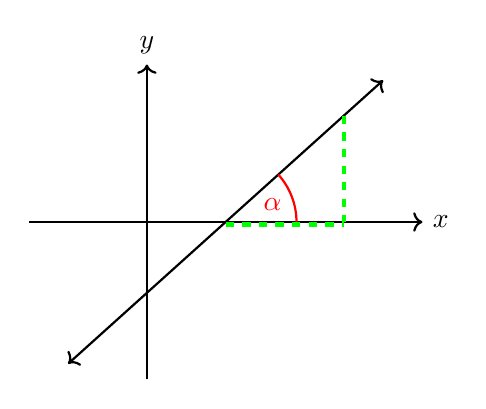
\begin{tikzpicture}

\coordinate (O) at (0,0);
\coordinate (x) at (3.5,0);
\coordinate (y) at (0,2);
\coordinate (A) at (3,1.8);
\coordinate (B) at (1.,0);
\coordinate (C) at (2.5,0);
\coordinate (D) at (-1,-1.8);

\draw[black,  thick, ->] (-1.5,0) --  (x) node[right] {$x$} ;
\draw[black,  thick, ->] (0,-2) --  (y) node[above] {$y$}  ;
\draw[black,  thick, <->] (D) --  (A)  ;
\draw[red, thick] (1.9,0) arc (0:{atan(0.9)}:.9) node [left, midway,xshift=0,yshift=-3] {$\alpha$};

\draw[green, ultra thick, dashed] (1,-.03) -- (2.5,-.03);
\draw[green, ultra thick, dashed] (2.5,1.35) -- (2.5,0);

\end{tikzpicture}
\newline




Section 4.2 Angle of inclination
\begin{tikzpicture}
\coordinate (O) at (0,0);
\coordinate (x) at (3.5,0);
\coordinate (y) at (0,2);
\coordinate (A) at (3,1.8);
\coordinate (B) at (1.,0);
\coordinate (C) at (2.5,0);
\coordinate (D) at (-1,-1.8);

\draw[black,  thick, ->] (-1.5,0) --  (x) node[right] {$x$} ;
\draw[black,  thick, ->] (0,-2) --  (y) node[above] {$y$}  ;
\draw[blue,  thick, <->] (D) --  (A)  ;
\draw[red, thick] (1.9,0) arc (0:{atan(0.9)}:.9) node [left, midway,xshift=0,yshift=-3] {$\alpha$};

\end{tikzpicture}
\newline



y=3/4 x - 3 
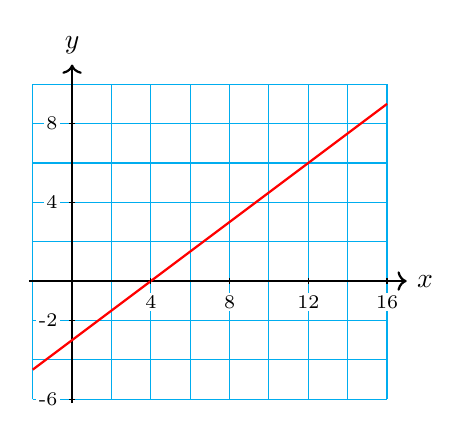
\begin{tikzpicture} [scale = 0.5]
\draw[cyan] (-1,-3) grid (8,5);

\coordinate (A) at (-1, -9/4);
\coordinate (B) at (8, 4.5);

\draw[black,  thick, ->] (-1.1,0) --  (8.5,0) node[right] {$x$} ;
\draw[black,  thick, ->] (0,-3.1) --  (0,5.5) node[above] {$y$}  ;
\draw[red,  thick] (B) --  (A)  ;

\foreach \x [evaluate=\x as \xi using int( 2* \x )] in {2, 4, 6, 8} \draw[black] ($ \x *(1,0) +(0,.08) $) --++(0,-.16) node[anchor=north, xshift=0,yshift=-3, fill=white, inner sep=1pt] {\scriptsize$ \xi $};

\foreach \y [evaluate=\y as \yi using int( 2* \y )]   in {-3, -1, 2, 4} \draw[black] (.08,\y ) --++(-.16,0) node[anchor=east, xshift=-3, fill=white, inner sep=1pt] {\scriptsize\yi};

\end{tikzpicture}
\newline



exam4-2-7 y= -6/5 x +2
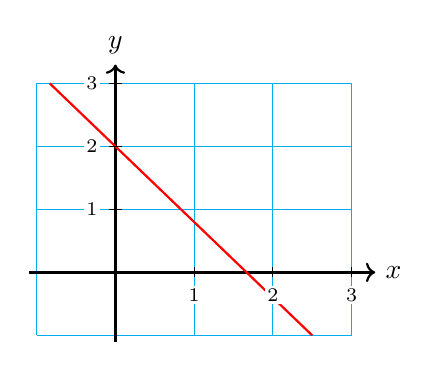
\begin{tikzpicture} [yscale=.8]
\draw[cyan] (-1,-1) grid (3,3);

\coordinate (A) at (-5/6, 3);
\coordinate (B) at (2.5,-1);

\draw[black,  thick, ->] (-1.1,0) --  (3.3,0) node[right] {$x$} ;
\draw[black,  thick, ->] (0,-1.1) --  (0,3.3) node[above] {$y$}  ;
\draw[red,  thick] (B) --  (A)  ;

\foreach \x [evaluate=\x as \xi using int( 1* \x )] in {1,2,3} \draw[black] ($ \x *(1,0) +(0,.08) $) --++(0,-.16) node[anchor=north, xshift=0,yshift=-3, fill=white, inner sep=1pt] {\scriptsize$ \xi $};

\foreach \y [evaluate=\y as \yi using int( 1* \y )]   in {1,2,3} \draw[black] (.08,\y ) --++(-.16,0) node[anchor=east, xshift=-3, fill=white, inner sep=1pt] {\scriptsize\yi};

\end{tikzpicture}
\newline



ar4-2-1 y= -6+ 2/3 x
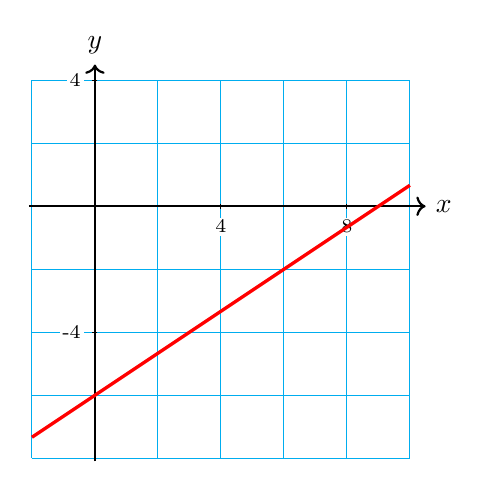
\begin{tikzpicture} [scale=.4]
\draw[cyan, xstep=2, ystep=2] (-2,-8) grid (10,4);

\draw[black, thick, ->] (-2.1,0) -- (10.5,0) node[right] {$x$} ;
\draw[black, thick, ->] (0,-8.1) -- (0,4.5) node[above] {$y$}  ;

\foreach \x [evaluate=\x as \xi using int( 1* \x )] in {4, 8} \draw[black] ($ \x *(1,0) +(0,.08) $) --++(0,-.16) node[anchor=north, xshift=0,yshift=-3, fill=white, inner sep=1pt] {\scriptsize$ \xi $};

\foreach \y [evaluate=\y as \yi using int( 1* \y )] in {-4, 4} \draw[black] (.08,\y ) --++(-.16,0) node[anchor=east, xshift=-3, fill=white, inner sep=1pt] {\scriptsize\yi};

\draw[domain=-2:10,smooth,variable=\x,red,very thick] plot ({\x},{-6+ 2/3 *\x)});
 \end{tikzpicture}
\newline



ar4-2-2 y= 4- 3/2 x
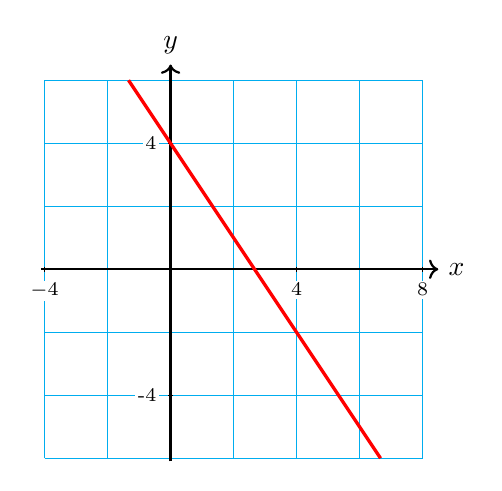
\begin{tikzpicture} [scale=.4]
\draw[cyan, xstep=2, ystep=2] (-4,-6) grid (8,6);

\draw[black, thick, ->] (-4.1,0) -- (8.5,0) node[right] {$x$} ;
\draw[black, thick, ->] (0,-6.1) -- (0,6.5) node[above] {$y$}  ;

\foreach \x [evaluate=\x as \xi using int( 1* \x )] in {-4, 4, 8} \draw[black] ($ \x *(1,0) +(0,.08) $) --++(0,-.16) node[anchor=north, xshift=0,yshift=-3, fill=white, inner sep=1pt] {\scriptsize$ \xi $};

\foreach \y [evaluate=\y as \yi using int( 1* \y )] in {-4, 4} \draw[black] (.08,\y ) --++(-.16,0) node[anchor=east, xshift=-3, fill=white, inner sep=1pt] {\scriptsize\yi};

\draw[domain={-4/3}:{20/3},smooth,variable=\x,red,very thick] plot ({\x},{4 - 3/2 *\x)});
 \end{tikzpicture}
\newline


ar4-2-3 $y= t^2 -4$
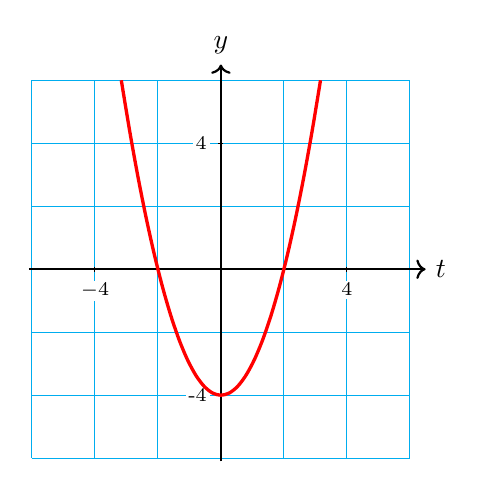
\begin{tikzpicture} [scale=.4]
\draw[cyan, xstep=2, ystep=2] (-6,-6) grid (6,6);

\draw[black, thick, ->] (-6.1,0) -- (6.5,0) node[right] {$t$} ;
\draw[black, thick, ->] (0,-6.1) -- (0,6.5) node[above] {$y$}  ;

\foreach \x [evaluate=\x as \xi using int( 1* \x )] in {-4, 4} \draw[black] ($ \x *(1,0) +(0,.08) $) --++(0,-.16) node[anchor=north, xshift=0,yshift=-3, fill=white, inner sep=1pt] {\scriptsize$ \xi $};

\foreach \y [evaluate=\y as \yi using int( 1* \y )] in {-4, 4} \draw[black] (.08,\y ) --++(-.16,0) node[anchor=east, xshift=-3, fill=white, inner sep=1pt] {\scriptsize\yi};

\draw[domain={-sqrt(10)}:{sqrt(10)},smooth,variable=\x,red,very thick] plot ({\x},{(\x)^2 -4});
 \end{tikzpicture}
\newline


ar4-2-4 $y= 9 -t^2 $
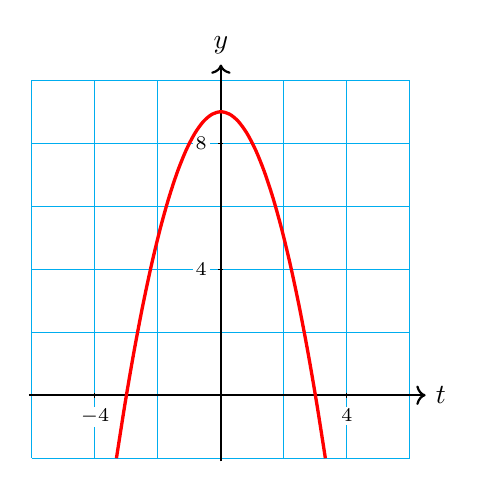
\begin{tikzpicture} [scale=.4]
\draw[cyan, xstep=2, ystep=2] (-6,-2) grid (6,10);

\draw[black, thick, ->] (-6.1,0) -- (6.5,0) node[right] {$t$} ;
\draw[black, thick, ->] (0,-2.1) -- (0,10.5) node[above] {$y$}  ;

\foreach \x [evaluate=\x as \xi using int( 1* \x )] in {-4, 4} \draw[black] ($ \x *(1,0) +(0,.08) $) --++(0,-.16) node[anchor=north, xshift=0,yshift=-3, fill=white, inner sep=1pt] {\scriptsize$ \xi $};

\foreach \y [evaluate=\y as \yi using int( 1* \y )] in {4, 8} \draw[black] (.08,\y ) --++(-.16,0) node[anchor=east, xshift=-3, fill=white, inner sep=1pt] {\scriptsize\yi};

\draw[domain={-sqrt(11)}:{sqrt(11)},smooth,variable=\x,red,very thick] plot ({\x},{9 - (\x)^2 });
 \end{tikzpicture}
\newline


ar4-2-5 $y= 2 -\sqrt{z} $
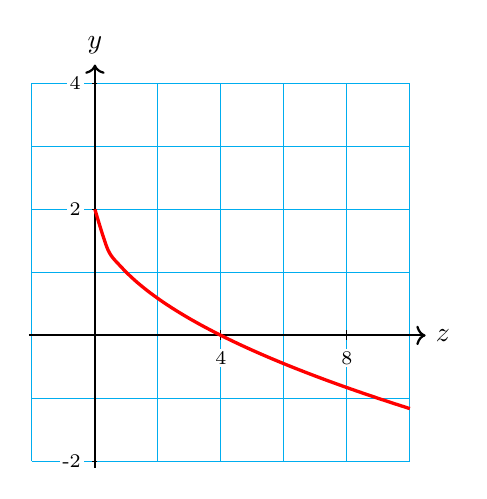
\begin{tikzpicture} [xscale=.4, yscale = .8]
\draw[cyan, xstep=2, ystep=1] (-2,-2) grid (10,4);

\draw[black, thick, ->] (-2.1,0) -- (10.5,0) node[right] {$z$} ;
\draw[black, thick, ->] (0,-2.1) -- (0,4.3) node[above] {$y$}  ;

\foreach \x [evaluate=\x as \xi using int( 1* \x )] in {4, 8} \draw[black] ($ \x *(1,0) +(0,.08) $) --++(0,-.16) node[anchor=north, xshift=0,yshift=-3, fill=white, inner sep=1pt] {\scriptsize$ \xi $};

\foreach \y [evaluate=\y as \yi using int( 1* \y )] in {-2, 2, 4} \draw[black] (.08,\y ) --++(-.16,0) node[anchor=east, xshift=-3, fill=white, inner sep=1pt] {\scriptsize\yi};

\draw[domain={0:10},smooth,variable=\x,red,very thick] plot ({\x},{2 - sqrt(\x) });
\end{tikzpicture}
\newline


ar4-2-6 $y= \sqrt{4-z} $
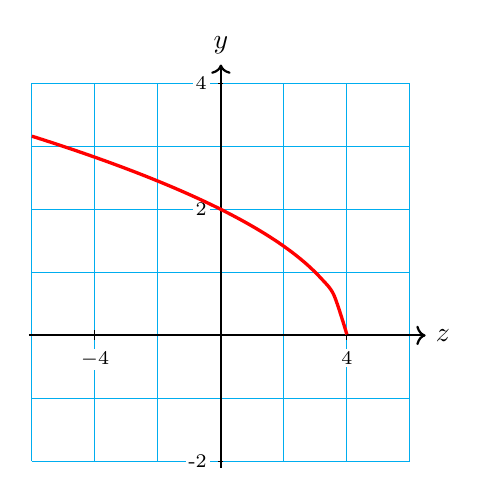
\begin{tikzpicture} [xscale=.4, yscale = .8]
\draw[cyan, xstep=2, ystep=1] (-6,-2) grid (6,4);

\draw[black, thick, ->] (-6.1,0) -- (6.5,0) node[right] {$z$} ;
\draw[black, thick, ->] (0,-2.1) -- (0,4.3) node[above] {$y$}  ;

\foreach \x [evaluate=\x as \xi using int( 1* \x )] in {-4, 4} \draw[black] ($ \x *(1,0) +(0,.08) $) --++(0,-.16) node[anchor=north, xshift=0,yshift=-3, fill=white, inner sep=1pt] {\scriptsize$ \xi $};

\foreach \y [evaluate=\y as \yi using int( 1* \y )] in {-2, 2, 4} \draw[black] (.08,\y ) --++(-.16,0) node[anchor=east, xshift=-3, fill=white, inner sep=1pt] {\scriptsize\yi};

\draw[domain={-6:4},smooth,variable=\x,red,very thick] plot ({\x},{sqrt(4-\x) });
\end{tikzpicture}
\newline


sq4-2-1 circle
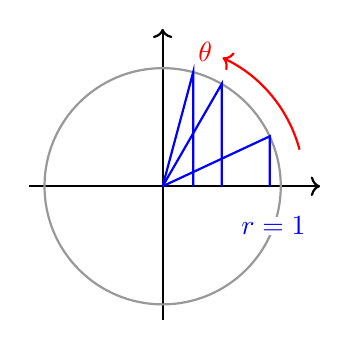
\begin{tikzpicture} 
\coordinate (O) at (0,0);
\coordinate (A) at (25:1.5);
\coordinate (Ap) at ($ 1.5*cos(25)*(1,0) $);
\coordinate (B) at (60:1.5);
\coordinate (Bp) at ($ 1.5*cos(60)*(1,0) $);
\coordinate (C) at (75:1.5);
\coordinate (Cp) at ($ 1.5*cos(75)*(1,0) $);

\draw[black, thick, ->] (-1.7,0) -- (2,0) ;
\draw[black, thick, ->] (0,-1.7) -- (0,2) ;

\draw[red, thick, ->] (15:1.8) arc(15:65:1.8) node[left,yshift=2]{$\theta$};

\draw[gray!80!white, thick] (O) circle (1.5cm);
\draw[blue, thick] (O)--(A)--(Ap);
\draw[blue, thick] (O)--(B)--(Bp);
\draw[blue, thick] (O)--(C)--(Cp);

\node[text width=1cm, text=blue,fill=white, inner sep=0pt] at (1.5,-.5)  {$r=1$};

\end{tikzpicture}
\newline


sq4-2-2 circle
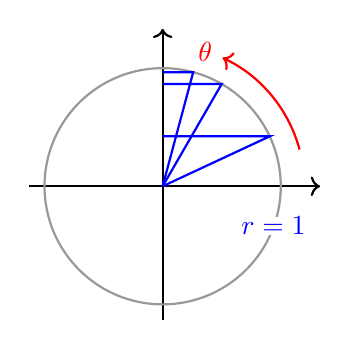
\begin{tikzpicture} 
\coordinate (O) at (0,0);
\coordinate (A) at (25:1.5);
\coordinate (Ap) at ($ 1.5*sin(25)*(0,1) $);
\coordinate (B) at (60:1.5);
\coordinate (Bp) at ($ 1.5*sin(60)*(0,1) $);
\coordinate (C) at (75:1.5);
\coordinate (Cp) at ($ 1.5*sin(75)*(0,1) $);

\draw[black, thick, ->] (-1.7,0) -- (2,0) ;
\draw[black, thick, ->] (0,-1.7) -- (0,2) ;

\draw[red, thick, ->] (15:1.8) arc(15:65:1.8) node[left,yshift=2]{$\theta$};

\draw[gray!80!white, thick] (O) circle (1.5cm);
\draw[blue, thick] (O)--(A)--(Ap);
\draw[blue, thick] (O)--(B)--(Bp);
\draw[blue, thick] (O)--(C)--(Cp);

\node[text width=1cm, text=blue,fill=white, inner sep=0pt] at (1.5,-.5)  {$r=1$};

\end{tikzpicture}
\newline


\section {Homework 4.2}

hp4-2-1 circle
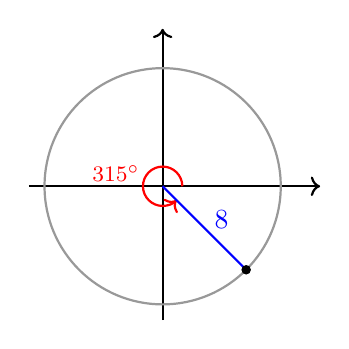
\begin{tikzpicture} 
\coordinate (O) at (0,0);
\coordinate (A) at (315:1.5);
\draw[black, thick, ->] (-1.7,0) -- (2,0) ;
\draw[black, thick, ->] (0,-1.7) -- (0,2) ;

\draw[red, thick, ->] (0.25,0) arc(0:315:.25) node[left, midway, xshift=2,yshift=2]{\footnotesize $315\degree$};

\draw[gray!80!white, thick] (O) circle (1.5cm);
\draw[blue, thick] (O)--(A) node[above right, midway, yshift=-4]{8};
\filldraw[black] (A) circle (1.5pt);

\end{tikzpicture}
\newline

hp4-2-2 circle
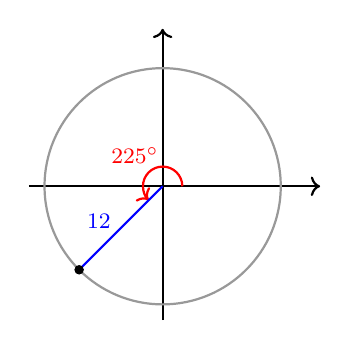
\begin{tikzpicture} 
\coordinate (O) at (0,0);
\coordinate (A) at (225:1.5);
\draw[black, thick, ->] (-1.7,0) -- (2,0) ;
\draw[black, thick, ->] (0,-1.7) -- (0,2) ;

\draw[red, thick, ->] (0.25,0) arc(0:225:.25) node[above left, midway, xshift=5, yshift=-2]{\footnotesize $225\degree$};

\draw[gray!80!white, thick] (O) circle (1.5cm);
\draw[blue, thick] (O)--(A) node[above left, midway, yshift=-4]{\footnotesize 12};
\filldraw[black] (A) circle (1.5pt);

\end{tikzpicture}
\newline

hp4-2-3 circle
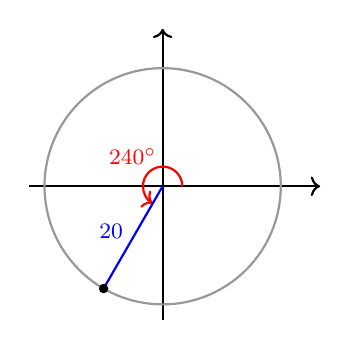
\begin{tikzpicture} 
\coordinate (O) at (0,0);
\coordinate (A) at (240:1.5);
\draw[black, thick, ->] (-1.7,0) -- (2,0) ;
\draw[black, thick, ->] (0,-1.7) -- (0,2) ;

\draw[red, thick, ->] (0.25,0) arc(0:240:.25) node[above left, midway, xshift=5, yshift=-2]{\footnotesize $240\degree$};

\draw[gray!80!white, thick] (O) circle (1.5cm);
\draw[blue, thick] (O)--(A) node[above left, midway, yshift=-4]{\footnotesize 20};
\filldraw[black] (A) circle (1.5pt);

\end{tikzpicture}
\newline

hp4-2-4 circle
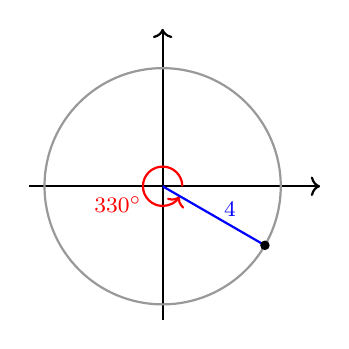
\begin{tikzpicture} 
\coordinate (O) at (0,0);
\coordinate (A) at (330:1.5);
\draw[black, thick, ->] (-1.7,0) -- (2,0) ;
\draw[black, thick, ->] (0,-1.7) -- (0,2) ;

\draw[red, thick, ->] (0.25,0) arc(0:330:.25) node[below left, midway, xshift=3, yshift=-2]{\footnotesize $330\degree$};

\draw[gray!80!white, thick] (O) circle (1.5cm);
\draw[blue, thick] (O)--(A) node[above right, midway, yshift=-4]{\footnotesize 4};
\filldraw[black] (A) circle (1.5pt);

\end{tikzpicture}
\newline

hp4-2-5 circle
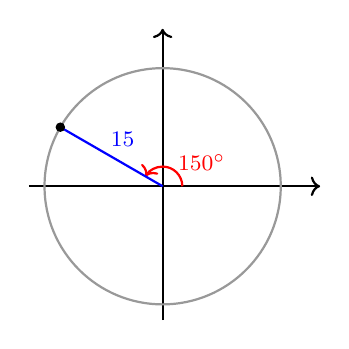
\begin{tikzpicture} 
\coordinate (O) at (0,0);
\coordinate (A) at (150:1.5);
\draw[black, thick, ->] (-1.7,0) -- (2,0) ;
\draw[black, thick, ->] (0,-1.7) -- (0,2) ;

\draw[red, thick, ->] (0.25,0) arc(0:150:.25) node[above right, midway, xshift=0, yshift=-5]{\footnotesize $150\degree$};

\draw[gray!80!white, thick] (O) circle (1.5cm);
\draw[blue, thick] (O)--(A) node[above right, midway, xshift=-4]{\footnotesize 15};
\filldraw[black] (A) circle (1.5pt);

\end{tikzpicture}
\newline

hp4-2-6 circle
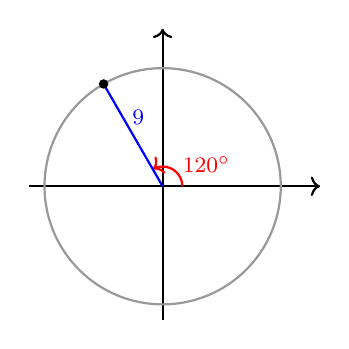
\begin{tikzpicture} 
\coordinate (O) at (0,0);
\coordinate (A) at (120:1.5);
\draw[black, thick, ->] (-1.7,0) -- (2,0) ;
\draw[black, thick, ->] (0,-1.7) -- (0,2) ;

\draw[red, thick, ->] (0.25,0) arc(0:120:.25) node[above right, midway, xshift=0, yshift=-5]{\footnotesize $120\degree$};

\draw[gray!80!white, thick] (O) circle (1.5cm);
\draw[blue, thick] (O)--(A) node[above right, midway, xshift=-4]{\footnotesize 9};
\filldraw[black] (A) circle (1.5pt);

\end{tikzpicture}
\newline

hp4-2-7 circle
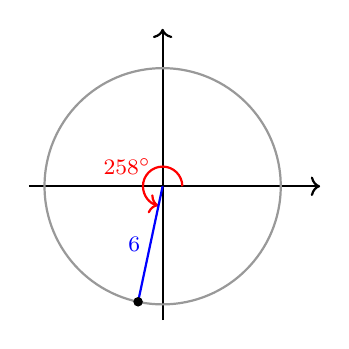
\begin{tikzpicture} 
\coordinate (O) at (0,0);
\coordinate (A) at (258:1.5);
\draw[black, thick, ->] (-1.7,0) -- (2,0) ;
\draw[black, thick, ->] (0,-1.7) -- (0,2) ;

\draw[red, thick, ->] (0.25,0) arc(0:258:.25) node[above left, midway, xshift=4, yshift=-5]{\footnotesize $258\degree$};

\draw[gray!80!white, thick] (O) circle (1.5cm);
\draw[blue, thick] (O)--(A) node[ left, midway, xshift=0]{\footnotesize 6};
\filldraw[black] (A) circle (1.5pt);

\end{tikzpicture}
\newline

hp4-2-8 circle
\begin{tikzpicture} 
\coordinate (O) at (0,0);
\coordinate (A) at (312:1.5);
\draw[black, thick, ->] (-1.7,0) -- (2,0) ;
\draw[black, thick, ->] (0,-1.7) -- (0,2) ;

\draw[red, thick, ->] (0.25,0) arc(0:312:.25) node[ left, midway, xshift=1, yshift=-10]{\footnotesize $312\degree$};

\draw[gray!80!white, thick] (O) circle (1.5cm);
\draw[blue, thick] (O)--(A) node[above right, midway, yshift=-3]{\footnotesize 16};
\filldraw[black] (A) circle (1.5pt);

\end{tikzpicture}
\newline

hp4-2-9 circle
\begin{tikzpicture} 
\coordinate (O) at (0,0);
\coordinate (A) at (296:1.5);
\draw[black, thick, ->] (-1.7,0) -- (2,0) ;
\draw[black, thick, ->] (0,-1.7) -- (0,2) ;

\draw[red, thick, ->] (0.25,0) arc(0:296:.25) node[above left, midway, xshift=4, yshift=0]{\footnotesize $296\degree$};

\draw[gray!80!white, thick] (O) circle (1.5cm);
\draw[blue, thick] (O)--(A) node[above right, midway, yshift=-5]{\footnotesize 13};
\filldraw[black] (A) circle (1.5pt);

\end{tikzpicture}
\newline

hp4-2-10 circle
\begin{tikzpicture} 
\coordinate (O) at (0,0);
\coordinate (A) at (341:1.5);
\draw[black, thick, ->] (-1.7,0) -- (2,0) ;
\draw[black, thick, ->] (0,-1.7) -- (0,2) ;

\draw[red, thick, ->] (0.25,0) arc(0:341:.25) node[ left, midway, xshift=2, yshift=-8]{\footnotesize $341\degree$};

\draw[gray!80!white, thick] (O) circle (1.5cm);
\draw[blue, thick] (O)--(A) node[below , midway, yshift=0]{\footnotesize 10};
\filldraw[black] (A) circle (1.5pt);

\end{tikzpicture}
\newline

hp4-2-11 circle
\begin{tikzpicture} 
\coordinate (O) at (0,0);
\coordinate (A) at (204:1.5);
\draw[black, thick, ->] (-1.7,0) -- (2,0) ;
\draw[black, thick, ->] (0,-1.7) -- (0,2) ;

\draw[red, thick, ->] (0.25,0) arc(0:204:.25) node[above left, midway, xshift=2, yshift=-4]{\footnotesize $204\degree$};

\draw[gray!80!white, thick] (O) circle (1.5cm);
\draw[blue, thick] (O)--(A) node[below , midway, yshift=0]{\footnotesize 20};
\filldraw[black] (A) circle (1.5pt);

\end{tikzpicture}
\newline

hp4-2-12 circle
\begin{tikzpicture} 
\coordinate (O) at (0,0);
\coordinate (A) at (106:1.5);
\draw[black, thick, ->] (-1.7,0) -- (2,0) ;
\draw[black, thick, ->] (0,-1.7) -- (0,2) ;

\draw[red, thick, ->] (0.25,0) arc(0:106:.25) node[above right, midway, xshift=0, yshift=-4]{\footnotesize $106\degree$};

\draw[gray!80!white, thick] (O) circle (1.5cm);
\draw[blue, thick] (O)--(A) node[left , midway, yshift=0]{\footnotesize 7};
\filldraw[black] (A) circle (1.5pt);

\end{tikzpicture}
\newline

fig-4-2-unitcircle
\begin{tikzpicture} [scale = .35] 
\draw[cyan] (-10,-10) grid (10,10);

\coordinate (O) at (0,0);

\draw[red,thick] (O) circle (10cm);
\foreach \theta  in {0,10,...,360}
\draw[black] (O)--(\theta:10)  ;

\foreach \x in {-10, -9, ..., 10} 
{
\draw[black,  thick] ($ \x *(1,0) +(0,.2) $) --++(0,-0.4); 
\draw[black,  thick] ($ \x *(0,1) +(.2,0) $) --++(-0.4,0); 
};

\foreach \x in {-10, -5, 5, 10} 
{
\draw[black, ultra thick] ($ \x *(1,0) +(0,.4) $) --++(0,-0.8); 
\draw[black, ultra thick] ($ \x *(0,1) +(.4,0) $) --++(-0.8,0); 
};

\foreach \theta  in {30, 60, 120, 150, 210, 240, 300, 330}
{
\draw[black] (O)--(\theta:10.4) ;
\node[text width=0.5cm, color=red,fill=white, inner sep=1pt] at (\theta:11.3) {\footnotesize $\theta\degree$};
};

\end{tikzpicture}
\newline

fig-4-2-circleandgraph

\begin{tikzpicture} [scale = .24] 
\draw[cyan] (-10,-10) grid (10,10);

\coordinate (O) at (0,0);

\draw[red,thick] (O) circle (10cm);
\foreach \theta  in {0,10,...,360}
\draw[black] (O)--(\theta:10)  ;

\foreach \x  in {-10, -9, ..., 10} 
{
\draw[black,  thick] ($ \x *(1,0) +(0,.2) $) --++(0,-0.4); 
\draw[black,  thick] ($ \x *(0,1) +(.2,0) $) --++(-0.4,0); 
};

\foreach \x  in {-10, -5, 5, 10} 
{
\draw[black, ultra thick] ($ \x *(1,0) +(0,.4) $) --++(0,-0.8); 
\draw[black, ultra thick] ($ \x *(0,1) +(.4,0) $) --++(-0.8,0); 
};

\foreach \theta  in {30, 60, 120, 150, 210, 240, 300, 330}
{
\draw[black] (O)--(\theta:10.4) ;
\node[text width=0.5cm, color=red,fill=white, inner sep=1pt] at (\theta:11.3) {\footnotesize $\theta\degree$};
};

\draw[cyan] (14,-10) grid (50,10);
\draw[black,very thick, ->] (14,0) --+(36.9,0) node[right]{$\theta$};
\foreach \x [evaluate=\x as \xi using int( 10*(\x - 14))] in {17, 20, ..., 50} 
{
\draw[black,  thick] ($ \x *(1,0) +(0,.2) $) --++(0,-0.4) node[anchor=north, yshift=-2,fill=white, inner sep=1pt]{\scriptsize$\xi \degree$}; 
};
\draw[black,very thick, ->] (14,-10) --(14,10.9);
\foreach \x  in {-10, -9, ..., 10} 
{
\draw[black,  thick] ($ \x *(0,1) +(14.2,0) $) --++(-0.4,0); 
};

\end{tikzpicture}
\newline

hp4-2-21ans sine graph

\begin{tikzpicture} [scale = .24] 
\draw[cyan] (0,-10) grid (36,10);
\draw[black,very thick, ->] (0,0) --+(36.9,0) node[right]{$\theta$};
\foreach \x [evaluate=\x as \xi using int( 10*(\x ))] in {9, 18, ..., 36} 
{
\draw[black,  thick] ($ \x *(1,0) +(0,.2) $) --++(0,-0.4) node[anchor=north, yshift=-2,fill=white, inner sep=1pt]{\scriptsize$\xi \degree$}; 
};
\draw[black,very thick, ->] (0,-10) --(0,10.9);
\foreach \x  in {-10, -9, ..., 10} 
{
\draw[black,  thick] ($ \x *(0,1) +(0.2,0) $) --++(-0.4,0); 
};
\draw[domain={0:36},smooth,variable=\x,red,very thick] plot ({\x},{ 10*sin(deg(\x *pi/18)) });

\end{tikzpicture}
\newline

hp4-2-23ans sine graph

\begin{tikzpicture} [xscale = .9, yscale = 1.25] 
\draw[cyan] (0,-1) grid (8,1);
\draw[black, thick, ->] (0,0) --+(8.4,0) node[right]{$\theta$};
\draw[black, thick, ->] (0,-1) --+(0,2.2);
\foreach \x [evaluate=\x as \xi using int( 45*(\x ))] in {2, 4, 6, 8} 
{
\draw[black,  thick] ($ \x *(1,0) +(0,.04) $) --++(0,-0.08) node[anchor=north, yshift=-2,fill=white, inner sep=1pt]{\scriptsize$\xi \degree$}; 
};
\foreach \y in {-1, 1} 
{
\draw[black,  thick] ($ (0, \y) +(.08,0) $) --++(-0.16, 0) node[anchor=east, xshift=-2,fill=white, inner sep=1pt]{\scriptsize \y }; 
};

\draw[domain={0:8},smooth,variable=\x,red,very thick] plot ({\x},{ sin(deg(\x *pi/4)) });

\end{tikzpicture}
\newline

hp4-2-25ans cosine graph

\begin{tikzpicture} [xscale = .6, yscale = 1.25] 
\draw[cyan] (0,-1) grid (12,1);
\draw[black, thick, ->] (0,0) --+(12.4,0) node[right]{$\theta$};
\draw[black, thick, ->] (0,-1) --+(0,2.2);
\foreach \x [evaluate=\x as \xi using int( 30*(\x ))] in {2, 4, ..., 12} 
{
\draw[black,  thick] ($ \x *(1,0) +(0,.04) $) --++(0,-0.08) node[anchor=north, yshift=-2,fill=white, inner sep=1pt]{\scriptsize$\xi \degree$}; 
};
\foreach \y in {-1, 1} 
{
\draw[black,  thick] ($ (0, \y) +(.08,0) $) --++(-0.16, 0) node[anchor=east, xshift=-2,fill=white, inner sep=1pt]{\scriptsize \y }; 
};

\draw[domain={0:12},smooth,variable=\x,red,very thick] plot ({\x},{ cos(deg(\x *pi/6)) });

\end{tikzpicture}
\newline

hp4-2-27 sine graph

\begin{tikzpicture} [scale = 1.25 ] 
\draw[cyan, xstep=0.5, ystep=0.2] (-4,-1) grid (4,1);
\draw[black, thick, ->] (-4,0) --+(8.3,0) node[right]{$\theta$};
\draw[black, thick, ->] (0,-1) --+(0,2.2);
\foreach \x [evaluate=\x as \xi using int( 90*(\x ))] in {-4, -1, 1, 3} 
{
\draw[black,  thick] ($ \x *(1,0) +(0,.04) $) --++(0,-0.08) node[anchor=north, yshift=-2,fill=white, inner sep=1pt]{\scriptsize$\xi \degree$}; 
};
\foreach \y in {-1, 1} 
{
\draw[black,  thick] ($ (0, \y) +(.08,0) $) --++(-0.16, 0) node[anchor=east, xshift=-2,fill=white, inner sep=1pt]{\scriptsize \y }; 
};

\draw[domain={-4:4},smooth,variable=\x,red,very thick] plot ({\x},{ sin(deg(\x *pi/2)) });

\coordinate (a) at ($ sin(-225) *(0,1) + (-2.5,0) $);
\coordinate (b) at ($ sin(-135)*(0,1) + (-1.5,0) $);
\coordinate (c) at ($ sin(-90)*(0,1) + (-1,0) $);
\coordinate (d) at ($ sin(45)*(0,1) + (0.5,0) $);
\coordinate (e) at ($ sin(180)*(0,1) + (2,0) $);
\coordinate (f) at ($ sin(315)*(0,1) + (3.5,0) $);

\filldraw[black] (a) circle (1.5pt) node[anchor=south west]{$a$};
\filldraw[black] (b) circle (1.5pt) node[anchor=north east]{$b$};
\filldraw[black] (c) circle (1.5pt) node[anchor=north]{$c$};
\filldraw[black] (d) circle (1.5pt) node[anchor=south east]{$d$};
\filldraw[black] (e) circle (1.5pt) node[anchor=north east]{$e$};
\filldraw[black] (f) circle (1.5pt) node[anchor=north west]{$f$};

\end{tikzpicture}
\newline

hp4-2-28 sine graph

\begin{tikzpicture} [scale = 1.25 ] 
\draw[cyan, xstep=0.3333, ystep=0.2] (-4,-1) grid (4,1);
\draw[black, thick, ->] (-4,0) --+(8.3,0) node[right]{$\theta$};
\draw[black, thick, ->] (0,-1) --+(0,2.2);
\foreach \x [evaluate=\x as \xi using int( 90*(\x ))] in {-4, -1, 1, 3} 
{
\draw[black,  thick] ($ \x *(1,0) +(0,.04) $) --++(0,-0.08) node[anchor=north, yshift=-2,fill=white, inner sep=1pt]{\scriptsize$\xi \degree$}; 
};
\foreach \y in {-1, 1} 
{
\draw[black,  thick] ($ (0, \y) +(.08,0) $) --++(-0.16, 0) node[anchor=east, xshift=-2,fill=white, inner sep=1pt]{\scriptsize \y }; 
};

\draw[domain={-4:4},smooth,variable=\x,red,very thick] plot ({\x},{ sin(deg(\x *pi/2)) });

\coordinate (a) at ($ sin(-270) *(0,1) + (-3,0) $);
\coordinate (b) at ($ sin(-210)*(0,1) + (-2.33,0) $);
\coordinate (c) at ($ sin(-60)*(0,1) + (-0.667,0) $);
\coordinate (d) at ($ sin(30)*(0,1) + (0.333,0) $);
\coordinate (e) at ($ sin(120)*(0,1) + (1.333,0) $);
\coordinate (f) at ($ sin(240)*(0,1) + (2.667,0) $);

\filldraw[black] (a) circle (1.5pt) node[anchor=south]{$a$};
\filldraw[black] (b) circle (1.5pt) node[anchor=south west]{$b$};
\filldraw[black] (c) circle (1.5pt) node[anchor=south east]{$c$};
\filldraw[black] (d) circle (1.5pt) node[anchor=north west]{$d$};
\filldraw[black] (e) circle (1.5pt) node[anchor=south west]{$e$};
\filldraw[black] (f) circle (1.5pt) node[anchor=north east]{$f$};

\end{tikzpicture}
\newline

hp4-2-29 cosine graph

\begin{tikzpicture} [scale = 1.25 ] 
\draw[cyan, xstep=0.3333, ystep=0.2] (-4,-1) grid (4,1);
\draw[black, thick, ->] (-4,0) --+(8.3,0) node[right]{$\theta$};
\draw[black, thick, ->] (0,-1) --+(0,2.2);
\foreach \x [evaluate=\x as \xi using int( 90*(\x ))] in {-4, -2, 2, 4} 
{
\draw[black,  thick] ($ \x *(1,0) +(0,.04) $) --++(0,-0.08) node[anchor=north, yshift=-2,fill=white, inner sep=1pt]{\scriptsize$\xi \degree$}; 
};
\foreach \y in {-1, 1} 
{
\draw[black,  thick] ($ (0, \y) +(.08,0) $) --++(-0.16, 0) node[anchor=east, xshift=-2,fill=white, inner sep=1pt]{\scriptsize \y }; 
};

\draw[domain={-4:4},smooth,variable=\x,red,very thick] plot ({\x},{ cos(deg(\x *pi/2)) });

\coordinate (a) at ($ cos(-240) *(0,1) + (-2.667,0) $);
\coordinate (b) at ($ cos(-210)*(0,1) + (-2.33,0) $);
\coordinate (c) at ($ cos(-60)*(0,1) + (-0.667,0) $);
\coordinate (d) at ($ cos(30)*(0,1) + (0.333,0) $);
\coordinate (e) at ($ cos(120)*(0,1) + (1.333,0) $);
\coordinate (f) at ($ cos(270)*(0,1) + (3,0) $);

\filldraw[black] (a) circle (1.5pt) node[anchor=north east]{$a$};
\filldraw[black] (b) circle (1.5pt) node[anchor=north east]{$b$};
\filldraw[black] (c) circle (1.5pt) node[anchor=south east]{$c$};
\filldraw[black] (d) circle (1.5pt) node[anchor=south west]{$d$};
\filldraw[black] (e) circle (1.5pt) node[anchor=north east]{$e$};
\filldraw[black] (f) circle (1.5pt) node[anchor=south east]{$f$};

\end{tikzpicture}
\newline

hp4-2-30 cosine graph

\begin{tikzpicture} [scale = 1.25 ] 
\draw[cyan, xstep=0.5, ystep=0.2] (-4,-1) grid (4,1);
\draw[black, thick, ->] (-4,0) --+(8.3,0) node[right]{$\theta$};
\draw[black, thick, ->] (0,-1) --+(0,2.2);
\foreach \x [evaluate=\x as \xi using int( 90*(\x ))] in {-4, -2, 2, 4} 
{
\draw[black,  thick] ($ \x *(1,0) +(0,.04) $) --++(0,-0.08) node[anchor=north, yshift=-2,fill=white, inner sep=1pt]{\scriptsize$\xi \degree$}; 
};
\foreach \y in {-1, 1} 
{
\draw[black,  thick] ($ (0, \y) +(.08,0) $) --++(-0.16, 0) node[anchor=east, xshift=-2,fill=white, inner sep=1pt]{\scriptsize \y }; 
};

\draw[domain={-4:4},smooth,variable=\x,red,very thick] plot ({\x},{ cos(deg(\x *pi/2)) });

\coordinate (a) at ($ cos(-315) *(0,1) + (-3.5,0) $);
\coordinate (b) at ($ cos(-135)*(0,1) + (-1.5,0) $);
\coordinate (c) at ($ cos(-90)*(0,1) + (-1,0) $);
\coordinate (d) at ($ cos(135)*(0,1) + (1.5,0) $);
\coordinate (e) at ($ cos(180)*(0,1) + (2,0) $);
\coordinate (f) at ($ cos(225)*(0,1) + (2.5,0) $);

\filldraw[black] (a) circle (1.5pt) node[anchor=south west]{$a$};
\filldraw[black] (b) circle (1.5pt) node[anchor=north east]{$b$};
\filldraw[black] (c) circle (1.5pt) node[anchor=north east]{$c$};
\filldraw[black] (d) circle (1.5pt) node[anchor=north east]{$d$};
\filldraw[black] (e) circle (1.5pt) node[anchor=north ]{$e$};
\filldraw[black] (f) circle (1.5pt) node[anchor=north west]{$f$};

\end{tikzpicture}
\newline

hp4-2-31ansb cosine graph

\begin{tikzpicture} [xscale = .9, yscale = 1.25] 
\draw[cyan] (0,-1) grid (8,1);
\draw[black, thick, ->] (0,0) --+(8.4,0) node[right]{$\theta$};
\draw[black, thick, ->] (0,-1) --+(0,2.2);
\foreach \x [evaluate=\x as \xi using int( 45*(\x ))] in {2, 4, 6, 8} 
{
\draw[black,  thick] ($ \x *(1,0) +(0,.04) $) --++(0,-0.08) node[anchor=north, yshift=-2,fill=white, inner sep=1pt]{\scriptsize$\xi \degree$}; 
};
\foreach \y in {-1, 1} 
{
\draw[black,  thick] ($ (0, \y) +(.08,0) $) --++(-0.16, 0) node[anchor=east, xshift=-2,fill=white, inner sep=1pt]{\scriptsize \y }; 
};

\draw[domain={0:8},smooth,variable=\x,red,very thick] plot ({\x},{ cos(deg(\x *pi/4)) });

\end{tikzpicture}
\newline

hp4-2-32a cosine graph
\begin{tikzpicture} 
\draw[black, thick, ->] (0,0) --+(3.3,0) node[right]{$\theta$};
\draw[black, thick, ->] (0,-1) --+(0,2.3) node[above]{$y$};
\draw[domain={0:pi},smooth,variable=\x,red,very thick] plot ({\x},{ cos(deg(\x *2)) });
\end{tikzpicture}
\newline

hp4-2-32b sine graph
\begin{tikzpicture} 
\draw[black, thick, ->] (0,0) --+(3.3,0) node[right]{$\theta$};
\draw[black, thick, ->] (0,-1) --+(0,2.3) node[above]{$y$};
\draw[domain={0:pi},smooth,variable=\x,red,very thick] plot ({\x},{ sin(deg(\x *2)) });
\end{tikzpicture}
\newline

hp4-2-32 combo graph
\begin{tikzpicture} 
\draw[black, thick, ->] (0,0) --+(3.3,0) node[right]{$\theta$};
\draw[black, thick, ->] (0,-1) --+(0,2.3) node[above]{$y$};
\draw[domain={0:pi},smooth,variable=\x,red,very thick] plot ({\x},{ cos(deg(\x *2)) });
\node[text width=.3cm] at (-0.5,0)  {a.};

\draw[black, thick, ->] (6,0) --+(3.3,0) node[right]{$\theta$};
\draw[black, thick, ->] (6,-1) --+(0,2.3) node[above]{$y$};
\draw[domain={6:pi+6},smooth,variable=\x,red,very thick] plot ({\x},{ sin(deg((\x - 6)*2)) });
\node[text width=.3cm] at (5.5,0)  {b.};

\end{tikzpicture}
\newline

fig-4-2-41 ferris wheel and graph

\begin{tikzpicture} [scale = .2] 
\coordinate (O) at (0,0);

\draw[black,thick] (-11.4,0) --(11.4,0);
\draw[black,thick] (0,-11.4) --(0,11.4);
\draw[red,thick] (O) circle (10cm);
\foreach \theta  in {0,15,...,360}
\draw[black] (O)--(\theta:10)  ;

\draw[cyan, xstep = 4, ystep = 5] (16,-10) grid (64,10);
\draw[black,thick, ->] (16,0) --+(48.9,0) node[right]{$\theta$};
\draw[black,thick, ->] (16,-10) --(16,11.5);

\draw[domain={16:64},smooth,variable=\x,red,very thick] plot ({\x},{ 10* sin(deg( (\x-16) *pi/24)) });

\coordinate (A) at (0:10);
\filldraw[black] (A) circle (0.4cm) node[anchor=north west]{$A$};
\coordinate (B) at (60:10);
\filldraw[black] (B) circle (0.4cm) node[anchor=south west]{$B$};
\coordinate (C) at (90:10);
\filldraw[black] (C) circle (0.4cm) node[anchor=south east]{$C$};
\coordinate (D) at (135:10);
\filldraw[black] (D) circle (0.4cm) node[anchor=east]{$D$};
\coordinate (E) at (210:10);
\filldraw[black] (E) circle (0.4cm) node[anchor=north east]{$E$};

\end{tikzpicture}
\newline

fig-4-2-41ans ferris wheel graph

\begin{tikzpicture} [scale = .2] 

\draw[cyan, xstep = 4, ystep = 5] (0,-10) grid (48,10);
\draw[black,thick, ->] (0,0) --+(48.9,0) node[right]{$\theta$};
\draw[black,thick, ->] (0,-10) --(0,11.5);

\draw[domain={0:48},smooth,variable=\x,red,very thick] plot ({\x},{ 10* sin(deg( (\x ) *pi/24)) });

\coordinate (A) at (0,0) ;
\filldraw[black] (A) circle (0.4cm) node[anchor=east]{$A$};
\coordinate (B) at ($ 10*sin(60)*(0,1) + (8,0) $);
\filldraw[black] (B) circle (0.4cm) node[anchor=south east]{$B$};
\coordinate (C) at ($ 10*sin(90)*(0,1) + (12,0) $);
\filldraw[black] (C) circle (0.4cm) node[anchor=south ]{$C$};
\coordinate (D) at ($ 10*sin(135)*(0,1) + (18,0) $);
\filldraw[black] (D) circle (0.4cm) node[anchor=north east]{$D$};
\coordinate (E) at ($ 10*sin(210)*(0,1) + (28,0) $);
\filldraw[black] (E) circle (0.4cm) node[anchor=north east]{$E$};

\end{tikzpicture}
\newline

fig-4-2-42 ferris wheel and graph

\begin{tikzpicture} [scale = .2] 
\coordinate (O) at (0,0);

\draw[black,thick] (-11.4,0) --(11.4,0);
\draw[black,thick] (0,-11.4) --(0,11.4);
\draw[red,thick] (O) circle (10cm);
\foreach \theta  in {0,15,...,360}
\draw[black] (O)--(\theta:10)  ;

\draw[cyan, xstep = 4, ystep = 5] (16,-10) grid (64,10);
\draw[black,thick, ->] (16,0) --+(48.9,0) node[right]{$\theta$};
\draw[black,thick, ->] (16,-10) --(16,11.5);

\draw[domain={16:64},smooth,variable=\x,red,very thick] plot ({\x},{ 10* sin(deg( (\x-16) *pi/24)) });

\coordinate (F) at ($ 10*sin(120)*(0,1)+(32,0) $);
\filldraw[black] (F) circle (0.4cm) node[anchor=south west]{$F$};
\coordinate (G) at (40,0);
\filldraw[black] (G) circle (0.4cm) node[anchor=north east]{$G$};
\coordinate (H) at ($ 10*sin(240)*(0,1) + (48,0) $);
\filldraw[black] (H) circle (0.4cm) node[anchor=north east]{$H$};
\coordinate (I) at (52,-10);
\filldraw[black] (I) circle (0.4cm) node[anchor=north, yshift=-1]{$I$};
\coordinate (J) at ($ 10*sin(315)*(0,1) + (58,0) $);
\filldraw[black] (J) circle (0.4cm) node[anchor=north west]{$J$};

\end{tikzpicture}
\newline

fig-4-2-43 circle and cosine graph

\begin{tikzpicture} [scale = .2] 
\coordinate (O) at (0,0);

\draw[black,thick] (-11.4,0) --(11.4,0);
\draw[black,thick] (0,-11.4) --(0,11.4);
\draw[red,thick] (O) circle (10cm);
\foreach \theta  in {0,15,...,360}
\draw[black] (O)--(\theta:10)  ;

\draw[cyan, xstep = 4, ystep = 5] (16,-10) grid (64,10);
\draw[black,thick, ->] (16,0) --+(48.9,0) node[right]{$\theta$};
\draw[black,thick, ->] (16,-10) --(16,11.5);

\draw[domain={16:64},smooth,variable=\x,red,very thick] plot ({\x},{ 10* cos(deg( (\x-16) *pi/24)) });

\coordinate (A) at (90:10);
\filldraw[black] (A) circle (0.4cm) node[anchor=south east]{$K$};
\coordinate (B) at (150:10);
\filldraw[black] (B) circle (0.4cm) node[anchor=south east]{$L$};
\coordinate (C) at (225:10);
\filldraw[black] (C) circle (0.4cm) node[anchor=north east]{$M$};
\coordinate (D) at (270:10);
\filldraw[black] (D) circle (0.4cm) node[anchor=north east]{$N$};
\coordinate (E) at (300:10);
\filldraw[black] (E) circle (0.4cm) node[anchor=north west]{$O$};

\end{tikzpicture}
\newline

fig-4-2-43ans cosine graph

\begin{tikzpicture} [scale = .2] 

\draw[cyan, xstep = 4, ystep = 5] (0,-10) grid (48,10);
\draw[black,thick, ->] (0,0) --+(48.9,0) node[right]{$\theta$};
\draw[black,thick, ->] (0,-10) --(0,11.5);

\draw[domain={0:48},smooth,variable=\x,red,very thick] plot ({\x},{ 10* cos(deg( (\x ) *pi/24)) });

\coordinate (A) at (0,10) ;
\filldraw[black] (A) circle (0.4cm) node[anchor=east]{$K$};
\coordinate (B) at ($ 10*cos(60)*(0,1) + (8,0) $);
\filldraw[black] (B) circle (0.4cm) node[anchor=south west]{$L$};
\coordinate (C) at ($ 10*cos(225)*(0,1) + (18,0) $);
\filldraw[black] (C) circle (0.4cm) node[anchor=north east ]{$M$};
\coordinate (D) at ($ 10*cos(180)*(0,1) + (24,0) $);
\filldraw[black] (D) circle (0.4cm) node[anchor=south ]{$N$};
\coordinate (E) at ($ 10*cos(210)*(0,1) + (28,0) $);
\filldraw[black] (E) circle (0.4cm) node[anchor=south ]{$O$};

\end{tikzpicture}
\newline

fig-4-2-44 circle and graph

\begin{tikzpicture} [scale = .2] 
\coordinate (O) at (0,0);

\draw[black,thick] (-11.4,0) --(11.4,0);
\draw[black,thick] (0,-11.4) --(0,11.4);
\draw[red,thick] (O) circle (10cm);
\foreach \theta  in {0,15,...,360}
\draw[black] (O)--(\theta:10)  ;

\draw[cyan, xstep = 4, ystep = 5] (16,-10) grid (64,10);
\draw[black,thick, ->] (16,0) --+(48.9,0) node[right]{$\theta$};
\draw[black,thick, ->] (16,-10) --(16,11.5);

\draw[domain={16:64},smooth,variable=\x,red,very thick] plot ({\x},{ 10* cos(deg( (\x-16) *pi/24)) });

\coordinate (F) at ($ 10*(0,1)+(16,0) $);
\filldraw[black] (F) circle (0.4cm) node[anchor=east]{$P$};
\coordinate (G) at ($ 10*cos(120)*(0,1) + (32,0) $);
\filldraw[black] (G) circle (0.4cm) node[anchor=north east]{$Q$};
\coordinate (H) at ($ 10*cos(210)*(0,1) + (44,0) $);
\filldraw[black] (H) circle (0.4cm) node[anchor=north west]{$R$};
\coordinate (I) at (52,0);
\filldraw[black] (I) circle (0.4cm) node[anchor=north west, yshift=-1]{$S$};
\coordinate (J) at ($ 10*cos(315)*(0,1) + (58,0) $);
\filldraw[black] (J) circle (0.4cm) node[anchor=north west]{$T$};

\end{tikzpicture}
\newline

hp4-2-45 circle on grid

\begin{tikzpicture} [scale = .4] 
\draw[cyan] (-10,-10) grid (10,10);
\draw[black, thick] (-10,0) -- (10,0);
\draw[black, thick] (0,-10) -- (0, 10);

\coordinate (O) at (0,0);

\draw[red,thick] (O) circle (10cm);

\foreach \x  in {-10, -9, ..., 10} 
{
\draw[black,  thick] ($ \x *(1,0) +(0,.2) $) --++(0,-0.4); 
\draw[black,  thick] ($ \x *(0,1) +(.2,0) $) --++(-0.4,0); 
};

\foreach \x  in {-10, -5, 5, 10} 
{
\draw[black, very thick] ($ \x *(1,0) +(0,.3) $) --++(0,-0.6); 
\draw[black, very thick] ($ \x *(0,1) +(.3,0) $) --++(-0.6,0); 
};

\filldraw[black] (10,0) circle (.5pt) node[anchor=north, yshift=-4, fill=white, inner sep=1pt, text=red] {1};
\filldraw[black] (0,10) circle (.5pt) node[anchor=east, xshift=-5, fill=white, inner sep=1pt, text=red] {1};

\node[text width=5.6cm] at (0,-11) {Use this grid for \#45 and \#46};

\end{tikzpicture}
\newline

hp4-2-45ans circle on grid

\begin{tikzpicture} [scale = .3] 
\draw[cyan, step=2] (-10,-10) grid (10,10);
\draw[black, thick] (-10,0) -- (10,0);
\draw[black, thick] (0,-10) -- (0, 10);

\coordinate (O) at (0,0);
\coordinate (A) at (10, 7.5);
\coordinate (B) at (-10, 7.5);

\draw[red,thick] (O) circle (10cm);

\filldraw[black] (10,0) circle (.5pt) node[anchor=north, yshift=-4, fill=white, inner sep=1pt, text=red] {1};
\filldraw[black] (0,10) circle (.5pt) node[anchor=east, xshift=-5, fill=white, inner sep=1pt, text=red] {1};

\draw[blue, thick, ->] (O)--(A);
\draw[blue, thick, ->] (O)--(B);
\draw[magenta, thick, ->] (3,0) arc(0:{atan(.75)}:3) node[right, midway, xshift=3,fill=white, inner sep=0pt]{$\alpha$};
\draw[black, thick, <->] (6,0) arc(0:{atan(.75)}:6) node[right, midway, xshift=5,fill=white, inner sep=0pt] {$\tilde{\alpha}$};
\draw[violet, thick, ->] (2,0) arc(0:{180-atan(.75)}:2) node[above, midway, xshift=-3, yshift=3,fill=white, inner sep=1pt]{$\beta$};
\draw[black, thick, <->] (-6,0) arc(180:{180-atan(.75)}:6) node[left, midway, xshift=-5,fill=white, inner sep=0pt] {$\tilde{\beta}$};

\draw[black, thick] (0.3,6) -- (-0.3,6) node[anchor=east, xshift=-3, fill=white, inner sep=1pt] {\footnotesize 0.6};
\draw[blue, ultra thick] (8,6)--(8,0)--(-8,0)--(-8,6)--(O)--(8,6);

\filldraw[black] (8,6) circle(.2cm);
\filldraw[black] (-8,6) circle(.2cm);

\end{tikzpicture}
\newline

hp4-2-47 circle on grid

\begin{tikzpicture} [scale = .4] 
\draw[cyan] (-10,-10) grid (10,10);
\draw[black, thick] (-10,0) -- (10,0);
\draw[black, thick] (0,-10) -- (0, 10);

\coordinate (O) at (0,0);

\draw[red,thick] (O) circle (10cm);

\foreach \x  in {-10, -9, ..., 10} 
{
\draw[black,  thick] ($ \x *(1,0) +(0,.2) $) --++(0,-0.4); 
\draw[black,  thick] ($ \x *(0,1) +(.2,0) $) --++(-0.4,0); 
};

\foreach \x  in {-10, -5, 5, 10} 
{
\draw[black, very thick] ($ \x *(1,0) +(0,.3) $) --++(0,-0.6); 
\draw[black, very thick] ($ \x *(0,1) +(.3,0) $) --++(-0.6,0); 
};

\filldraw[black] (10,0) circle (.5pt) node[anchor=north, yshift=-4, fill=white, inner sep=1pt, text=red] {1};
\filldraw[black] (0,10) circle (.5pt) node[anchor=east, xshift=-5, fill=white, inner sep=1pt, text=red] {1};

\node[text width=5.6cm] at (0,-11) {Use this grid for \#47 and \#48};

\end{tikzpicture}
\newline

hp4-2-47ans circle on grid

\begin{tikzpicture} [scale = .3] 
\draw[cyan, step=2] (-10,-10) grid (10,10);
\draw[black, thick] (-10,0) -- (10,0);
\draw[black, thick] (0,-10) -- (0, 10);

\coordinate (O) at (0,0);
\coordinate (A) at ({acos(0.3)}:11);
\coordinate (B) at ({360-acos(0.3)}:11);
\coordinate (C) at ({acos(0.3)}:10);
\coordinate (D) at ({-acos(0.3)}:10);

\draw[blue, very thick] (O)--(C)--(D)--(O)--+(3,0);

\draw[red,thick] (O) circle (10cm);

\filldraw[black] (10,0) circle (.5pt) node[anchor=north, yshift=-4, fill=white, inner sep=1pt, text=red] {1};
\filldraw[black] (0,10) circle (.5pt) node[anchor=east, xshift=-5, fill=white, inner sep=1pt, text=red] {1};

\draw[blue, thick, ->] (O)--(A);
\draw[blue, thick, ->] (O)--(B);
\draw[magenta, thick, ->] (4,0) arc(0:{acos(.3)}:4) node[right, midway, xshift=3,fill=white, inner sep=0pt]{$\alpha$};
\draw[black, thick, <->] (6,0) arc(0:{acos(.3)}:6) node[right, midway, xshift=5,fill=white, inner sep=0pt] {$\tilde{\alpha}$};
\draw[violet, thick, ->] (2,0) arc(0:{360-acos(.3)}:2) node[above, midway, xshift=-3, yshift=3,fill=white, inner sep=1pt]{$\beta$};
\draw[black, thick, <->] (6,0) arc(0:{-acos(.3)}:6) node[right, midway, xshift=5,fill=white, inner sep=0pt] {$\tilde{\beta}$};

\draw[black, thick] (3,.3) -- (3,-.3) node[anchor=north, yshift=-3, fill=white, inner sep=0pt] {\footnotesize 0.3};

\filldraw[black] (6,-8) circle(.2cm);
\filldraw[black] (-6,-8) circle(.2cm);

\end{tikzpicture}
\newline


fig-4-2-sinegraph sine graph

\begin{tikzpicture} [xscale=1.2, yscale=2]

\draw[cyan,xstep=pi/9,ystep=0.2]
(0,-1) grid (2*pi,1);

\draw[->] (-0.3,0) -- (6.5,0) node[right] {\footnotesize$\theta$};
\draw[->] (0,-0.2) -- (0,1.2) node[above] {\footnotesize$y=\sin(\theta)$};

\foreach \x [evaluate=\x as \xi using int( 20*(\x ))]  in {2, 4,...,18}
\draw[black] ($ pi*\x /9*(1,0) +(0,.04) $) --++(0,-.08) node[anchor=north, yshift=-4, fill=white, inner sep=0pt] {\scriptsize \xi};
\foreach \y   in {-1, -.8, ..., -.2, .2, .4,..., 1}
\draw[black] (.08,\y ) --++(-.16,0) ;
\foreach \y in {-1,1}
\draw[black, thick] (.12,\y ) --++(-.24,0) node[anchor=east] {\footnotesize \y};

\draw[domain=0:2*pi,smooth,variable=\x,red,very thick] plot ({\x},{sin(deg(\x))});

\end{tikzpicture}
\newline


fig-4-2-cosinegraph cosine graph

\begin{tikzpicture} [xscale=1.2, yscale=2]

\draw[cyan,xstep=pi/9,ystep=0.2]
(0,-1) grid (2*pi,1);

\draw[->] (-0.3,0) -- (6.5,0) node[right] {\footnotesize$\theta$};
\draw[->] (0,-0.2) -- (0,1.2) node[above] {\footnotesize$y=\cos(\theta)$};

\foreach \x [evaluate=\x as \xi using int( 20*(\x ))]  in {2, 4,...,18}
\draw[black] ($ pi*\x /9*(1,0) +(0,.04) $) --++(0,-.08) node[anchor=north, yshift=-4, fill=white, inner sep=0pt] {\scriptsize \xi};
\foreach \y   in {-1, -.8, ..., -.2, .2, .4,..., 1}
\draw[black] (.08,\y ) --++(-.16,0) ;
\foreach \y in {-1,1}
\draw[black, thick] (.12,\y ) --++(-.24,0) node[anchor=east] {\footnotesize \y};

\draw[domain=0:2*pi,smooth,variable=\x,red,very thick] plot ({\x},{cos(deg(\x))});

\end{tikzpicture}
\newline



hp4-2-58 grid

\begin{tikzpicture} [xscale=1.6, yscale=.25]
\draw[cyan,xstep=0.3333, ystep=2]
(0,-10) grid (4,10);

\draw[->] (-.1,0) -- (4.2,0) node[right] {$\theta$};
\draw[->] (0,-10.2) -- (0,10.9) node[above] {$y$};

\foreach \x [evaluate=\x as \xi using int( 90* \x )] in {1,2,...,4}
\draw[black] ($ \x *(1,0) +(0,.8) $) --++(0,-1.6) node[anchor=north, xshift=0,yshift=-3, fill=white, inner sep=1pt] {\scriptsize$ \xi $};

\foreach \y in {-10, -8,...,-2,2, 4, ...,10}
\draw[black] (.08,\y ) --++(-.16,0) node[anchor=east, xshift=-3, fill=white, inner sep=1pt] {\scriptsize\y};

\end{tikzpicture}
\newline


hp4-2-59ans tangent graph

\begin{tikzpicture} [xscale=.9,yscale=.5]
\draw[cyan] (-4,-5) grid (4,5);

\draw[->] (-.1,0) -- (4.2,0) node[right] {$\theta$};
\draw[->] (0,-5.1) -- (0,5.5);
\foreach \x [evaluate=\x as \xi using int( 45* \x )] in {-4, -2, 2, 4} \draw[black] ($ \x *(1,0) +(0,.08) $) --++(0,-.16) node[anchor=north, xshift=0,yshift=-3, fill=white, inner sep=1pt] {\scriptsize$ \xi $};

\foreach \y [evaluate=\y as \yi using int( 2* \y )]   in {-4,-2, 2,4} \draw[black] (.08,\y ) --++(-.16,0) node[anchor=east, xshift=-3, fill=white, inner sep=1pt] {\scriptsize\yi};

\draw[domain={atan(-5)/45:atan(5)/45},smooth,variable=\x,red,very thick] plot ({\x},{tan(45*\x)});

\draw[domain={atan(-5)/45+4:4},smooth,variable=\x,red,very thick] plot ({\x},{tan(45*\x)});

\draw[domain={-4:atan(5)/45-4},smooth,variable=\x,red,very thick] plot ({\x},{tan(45*\x)});

\end{tikzpicture}
\newline


hp4-2-69ans tangent graph

\begin{tikzpicture} [xscale=.6, yscale=.3]
\draw[cyan] (0,-10) grid (12,10);

\draw[->] (-.1,0) -- (12.5,0) node[right] {$\alpha$};
\draw[->] (0,-10.1) -- (0,10.5) node[anchor=south]{$m$};
\foreach \x [evaluate=\x as \xi using int( 15* \x )] in {2, 4, ..., 12} \draw[black] ($ \x *(1,0) +(0,.08) $) --++(0,-.16) node[anchor=north, xshift=0,yshift=-3, fill=white, inner sep=1pt] {\scriptsize$ \xi $};

\foreach \y   in {-10, -5, 5, 10} \draw[black] (.08,\y ) --++(-.16,0) node[anchor=east, xshift=-3, fill=white, inner sep=1pt] {\scriptsize\y};

\draw[domain={0:atan(10)/15},smooth,variable=\x,red,very thick] plot ({\x},{tan(15*\x)});

\draw[domain={atan(-10)/15+12:12},smooth,variable=\x,red,very thick] plot ({\x},{tan(15*\x)});


\end{tikzpicture}
\newline









\section {Stuff for later}



On a unit circle
\begin{tikzpicture} [scale=1.7]

\draw[thick,->] (-1.2,0) -- (1.3,0) node[anchor=west] {$x$};
\draw[thick,->] (0,-1.2) -- (0,1.3) node[anchor=south] {$y$};

\coordinate(O) at (0,0);
\coordinate(A) at (1,0);
\coordinate (B) at (-.6428,0.766);

\draw[gray,thick] (O) circle (1);
\draw[blue,thick] (O) -- (B) node[below left, midway, xshift=2, yshift=4] {\small\color{blue} $r=1$};
\filldraw [blue] (A) circle (1pt);
\filldraw [blue] (B) circle (1pt);
\draw[blue,thick] (A) arc(0:130:1) node[above, midway, xshift=14, yshift=-8] {\color{blue}$s$};
\draw[red,thick] (O)++(.2,0) arc(0:130:.2) node[above, midway, xshift=4, yshift=-3] {\color{blue}$\theta$};

\end{tikzpicture}
\newline



sine graph
\begin{tikzpicture}

\draw[cyan,xstep=pi/12,ystep=0.18]
(-2*pi,-1.8) grid (2*pi,1.8);

\draw[->] (-6.3,0) -- (6.5,0) node[right] {$\theta$};
\draw[->] (0,-1.8) -- (0,2.2) node[above] {$f(\theta)=\sin(\theta)$};

\foreach \x in {-24,-23,...,24}
\draw[black] ($ pi*\x /12*(1,0) +(0,.08) $) --++(0,-.16);
\foreach \y in {-0.9, 0.9}
\draw[black] (.08,\y ) --++(-.16,0);
\foreach \y in {-1,1}
\draw[black, thick] (.12,1.8*\y ) --++(-.24,0) node[anchor=east, xshift=-3, fill=white, inner sep=1pt] {\y};

\draw[black, thick] (-2*pi,.2) --++(0,-.4) node[anchor=north, xshift=-2,yshift=-3, fill=white, inner sep=1pt] {$-2\pi$};
\draw[black, thick] (2*pi,.2) --++(0,-.4) node[anchor=north, xshift=2,yshift=-3, fill=white, inner sep=1pt] {$2\pi$};

\draw[black] (pi,.2) --++(0,-.4) node[anchor=north, yshift=-3, fill=white, inner sep=1pt] {$\pi$};

\draw[black] (pi,.2) --++(0,-.4) node[anchor=north, yshift=-3, fill=white, inner sep=1pt] {$\pi$};
\draw[black] (-pi,.2) --++(0,-.4) node[anchor=north, xshift=-2,yshift=-3, fill=white, inner sep=1pt] {$-\pi$};
\draw[black] (-pi/2,.15) --++(0,-.3) node[anchor=north, yshift=-3, fill=white, inner sep=1pt] {$\frac{-\pi}{2}$};
\draw[black] (pi/2,.15) --++(0,-.3) node[anchor=north, yshift=-3, fill=white, inner sep=1pt] {$\frac{\pi}{2}$};
\draw[black] (3*pi/2,.15) --++(0,-.3) node[anchor=north, yshift=-3, fill=white, inner sep=1pt] {$\frac{3\pi}{2}$};
\draw[black] (-3*pi/2,.15) --++(0,-.3) node[anchor=north, yshift=-3, fill=white, inner sep=1pt] {$\frac{-3\pi}{2}$};

\draw[black] (pi/4,.11) --++(0,-.22) node[anchor=north, yshift=-4, fill=white, inner sep=1pt] {$\frac{\pi}{4}$};

\draw[black] (3*pi/4,.11) --++(0,-.22) node[anchor=north, yshift=-3, fill=white, inner sep=1pt] {$\frac{3\pi}{4}$};

\draw[domain=-2*pi:2*pi,smooth,variable=\x,red,very thick] plot ({\x},{1.8*sin(deg(\x))});

\end{tikzpicture}
\newline


cosine graph
\begin{tikzpicture} 

\draw[cyan,xstep=pi/12,ystep=0.18]
(-2*pi,-1.8) grid (2*pi,1.8);

\draw[->] (-6.3,0) -- (6.5,0) node[right] {$\theta$};
\draw[->] (0,-1.8) -- (0,2.2) node[above] {$f(\theta)=\cos(\theta)$};

\foreach \x in {-24,-23,...,24}
\draw[black] ($ pi*\x /12*(1,0) +(0,.08) $) --++(0,-.16);
\foreach \y in {-0.9, 0.9}
\draw[black] (.08,\y ) --++(-.16,0);
\foreach \y in {-1,1}
\draw[black, thick] (.12,1.8*\y ) --++(-.24,0) node[anchor=east, xshift=-3, fill=white, inner sep=1pt] {\y};

\draw[black, thick] (-2*pi,.2) --++(0,-.4) node[anchor=north, xshift=-2,yshift=-3, fill=white, inner sep=1pt] {$-2\pi$};
\draw[black, thick] (2*pi,.2) --++(0,-.4) node[anchor=north, xshift=2,yshift=-3, fill=white, inner sep=1pt] {$2\pi$};

\draw[black] (pi,.2) --++(0,-.4) node[anchor=north, yshift=-3, fill=white, inner sep=1pt] {$\pi$};

\draw[black] (pi,.2) --++(0,-.4) node[anchor=north, yshift=-3, fill=white, inner sep=1pt] {$\pi$};
\draw[black] (-pi,.2) --++(0,-.4) node[anchor=north, xshift=-2,yshift=-3, fill=white, inner sep=1pt] {$-\pi$};
\draw[black] (-pi/2,.15) --++(0,-.3) node[anchor=north, yshift=-3, fill=white, inner sep=1pt] {$\frac{-\pi}{2}$};
\draw[black] (pi/2,.15) --++(0,-.3) node[anchor=north, yshift=-3, fill=white, inner sep=1pt] {$\frac{\pi}{2}$};
\draw[black] (3*pi/2,.15) --++(0,-.3) node[anchor=north,xshift=3, yshift=-3, fill=white, inner sep=1pt] {$\frac{3\pi}{2}$};
\draw[black] (-3*pi/2,.15) --++(0,-.3) node[anchor=north,xshift=-3, yshift=-3, fill=white, inner sep=1pt] {$\frac{-3\pi}{2}$};

\draw[black] (pi/4,.11) --++(0,-.22) node[anchor=north, yshift=-4, fill=white, inner sep=1pt] {$\frac{\pi}{4}$};

\draw[black] (3*pi/4,.11) --++(0,-.22) node[anchor=north, yshift=-3, fill=white, inner sep=1pt] {$\frac{3\pi}{4}$};

\draw[black] (5*pi/4,.11) --++(0,-.22) node[anchor=north, yshift=-3, fill=white, inner sep=1pt] {$\frac{5\pi}{4}$};

\draw[domain=-2*pi:2*pi,smooth,variable=\x,red,very thick] plot ({\x},{1.8*cos(deg(\x))});

\end{tikzpicture}
\newline


tangent graph
\begin{tikzpicture} [yscale=.5]

\draw[cyan,xstep=pi/12,ystep=0.5]
(-2*pi,-5) grid (2*pi,5);

\draw[->] (-6.3,0) -- (6.5,0) node[right] {$\theta$};
\draw[->] (0,-5) -- (0,5.5) node[above] {$f(\theta)=\tan(\theta)$};

\foreach \x in {-24,-23,...,24}
\draw[black] ($ pi*\x /12*(1,0) +(0,.08) $) --++(0,-.16);
\foreach \y in {-5,-4,...,-1,1,2,...,5}
\draw[black, thick] (.10,\y ) --++(-.2,0) node[anchor=east, xshift=-3, fill=white, inner sep=1pt] {\y};

\draw[black, thick] (-2*pi,.2) --++(0,-.4) node[anchor=north, xshift=-2,yshift=-3, fill=white, inner sep=1pt] {$-2\pi$};
\draw[black, thick] (2*pi,.2) --++(0,-.4) node[anchor=north, xshift=2,yshift=-3, fill=white, inner sep=1pt] {$2\pi$};

\draw[black] (pi,.2) --++(0,-.4) node[anchor=north, yshift=-3, fill=white, inner sep=1pt] {$\pi$};

\draw[black] (pi,.2) --++(0,-.4) node[anchor=north, yshift=-3, fill=white, inner sep=1pt] {$\pi$};
\draw[black] (-pi,.2) --++(0,-.4) node[anchor=north, xshift=-2,yshift=-3, fill=white, inner sep=1pt] {$-\pi$};
\draw[black] (-pi/2,.15) --++(0,-.3) node[anchor=north, yshift=-3, fill=white, inner sep=1pt] {$\frac{-\pi}{2}$};
\draw[black] (pi/2,.15) --++(0,-.3) node[anchor=north, yshift=-3, fill=white, inner sep=1pt] {$\frac{\pi}{2}$};
\draw[black] (3*pi/2,.15) --++(0,-.3) node[anchor=north,xshift=3, yshift=-3, fill=white, inner sep=1pt] {$\frac{3\pi}{2}$};
\draw[black] (-3*pi/2,.15) --++(0,-.3) node[anchor=north,xshift=-3, yshift=-3, fill=white, inner sep=1pt] {$\frac{-3\pi}{2}$};

\draw[black] (pi/4,.11) --++(0,-.22) node[anchor=north, yshift=-4, fill=white, inner sep=1pt] {$\frac{\pi}{4}$};

\draw[black] (3*pi/4,.11) --++(0,-.22) node[anchor=north, yshift=-3, fill=white, inner sep=1pt] {$\frac{3\pi}{4}$};

\draw[black] (5*pi/4,.11) --++(0,-.22) node[anchor=north, yshift=-3, fill=white, inner sep=1pt] {$\frac{5\pi}{4}$};

\foreach \i in {-1, 0, 1}
	\draw[domain={\i*pi-atan(5)*pi/180}:{\i*pi+atan(5)*pi/180}, smooth, variable=\x,red,very thick] plot ({\x},{tan(deg(\x))}) ;

\draw[domain={-2*pi:atan(5)*pi/180-2*pi}, smooth, variable=\x,red,very thick] plot ({\x},{tan(deg(\x))}) ;
\draw[domain={2*pi-atan(5)*pi/180:2*pi}, smooth, variable=\x,red,very thick] plot ({\x},{tan(deg(\x))}) ;

\end{tikzpicture}
\newline


part A: law of sines a circumscribing circle

\begin{tikzpicture} [scale=.4]

\coordinate (O) at (0,0);
\coordinate (A) at (-3,-4);
\coordinate (B) at (3,-4);
\coordinate (C) at (-1.92,4.62);

\filldraw (A) circle (.1cm) node[anchor=north east] {$A$};
\filldraw (B) circle (.1cm) node[anchor=north west] {$B$};
\filldraw (C) circle (.1cm) node[anchor=south east] {$C$};

\draw[black,thick] (A)--(B)--(C)--(A);
\draw[gray!40!white, thick, dashed](O)++(0,1) -- (0,-4)--+(0,-.5);
\draw[gray!40!white, thick, dashed](O)++(.862,-.108) -- (-2.96,.31)--++(-.862,.108);
\draw[blue!80!white,thick] (0,-4)++(.75,0)-- ++(0,.75) -- ++(-.75,0);
\draw[blue!80!white,thick] (-2.46,.31) ++(.0864,.6896) -- ++(.6896,-.0864) -- ++(-.0864,-.6896);
\filldraw (O) circle (.2cm) node[anchor=north east] {$O$};

\draw[blue] (O) circle (5);

\end{tikzpicture}
\newline

part B: law of sines a circumscribing circle

\begin{tikzpicture} [scale=.4]

\coordinate (O) at (0,0);
\coordinate (A) at (-3,-4);
\coordinate (B) at (3,-4);
\coordinate (C) at (-1.92,4.62);
\coordinate (Cp) at (-4.62,1.92);
\coordinate (Cpp) at (0,5);
\coordinate (Cppp) at (3,4);
\coordinate (Cpppp) at (5,0);

\filldraw (O) circle (.1cm) node[anchor=north east] {$O$};
\filldraw (A) circle (.1cm) node[anchor=north east] {$A$};
\filldraw (B) circle (.1cm) node[anchor=north west] {$B$};
\filldraw (C) circle (.1cm) node[anchor=south east] {$C$};

\draw[draw= blue, fill=blue!80!white] (A)--(B)--(C)--(A);
\draw[draw= blue, fill=blue!30!white, opacity=.5] (A)--(B)--(Cp)--(A);
\draw[draw= blue, fill=blue!30!white, opacity=.5] (A)--(B)--(Cpp)--(A);
\draw[draw= blue, fill=blue!30!white, opacity=.5] (A)--(B)--(Cppp)--(A);
\draw[draw= blue, fill=blue!30!white, opacity=.5] (A)--(B)--(Cpppp)--(A);


\draw[blue] (O) circle (5);

\end{tikzpicture}
\newline

Exercise not used?
\begin{tikzpicture}
\coordinate (O) at (0,0);
\coordinate (A) at (0,0);
\coordinate (B) at (0,0);
\coordinate(C) at (0,0);
\coordinate (D) at (0,0);
\filldraw[black] (O) circle (.2pt) node[anchor=south west, xshift=6]{$50\degree$};
\filldraw[black] (A) circle (.2pt) node[anchor=south east]{$x$};
\filldraw[black] (B) circle (.2pt) node[anchor=north east, xshift=-6]{$y$};
\filldraw[black] (C) circle (.2pt) node[anchor=north west]{$z$};
%\draw[black,  thick] (A) -- (B) --( C) -- cycle;
\draw[black] (-2.3,0) --  (2.3,0);
\draw[black] (0.8,1.3) --  (-0.8,-1.3) ;
\end{tikzpicture}
\newline


\end{document}
